
%----------------------------------------------------------------------------------------

\documentclass[
	a4paper, % Paper size, use either a4paper or letterpaper
	12pt, % Default font size, the template is designed to look good at 12pt so it's best not to change this
	%unnumberedsections, % Uncomment for no section numbering
]{CSSullivanBusinessReport}



%----------------------------------------------------------------------------------------
%	REPORT INFORMATION
%----------------------------------------------------------------------------------------
\reportsubtitle{CSE-406 Project} % Report subtitle, include new lines if needed

\reporttitle{Burp Suite Documentation} % The report title to appear on the title page and page headers, do not create manual new lines here as this will carry over to page headers



\reportauthors{\textbf{Submitted by:}
\\\smallskip \textit{Udayon Paul Dhrubo(1805109)}
\\\smallskip \textit{Anika Monir(1805110)}} % Report authors/group/department, include new lines if neededa

\reportdate{\today} % Report date, include new lines for additional information if needed

\rightheadercontent{
\includegraphics[width=3cm]{Images/burpsuite.png}} % The content in the right header, you may want to add your own company logo or use your company/department name or leave this command empty for no right header content

%----------------------------------------------------------------------------------------

\setcounter{tocdepth}{4}
\setcounter{secnumdepth}{4}
\begin{document}

%----------------------------------------------------------------------------------------
%	TITLE PAGE
%----------------------------------------------------------------------------------------

\thispagestyle{empty} % Suppress headers and footers on this page

\begin{fullwidth} % Use the whole page width
	\vspace*{-0.075\textheight} % Pull logo into the top margin
	
	\hfill 
\includegraphics[width=5cm]{Images/burpsuite.png} % Company logo

	\vspace{0.15\textheight} % Vertical whitespace

	\parbox{0.9\fulltextwidth}{\fontsize{50pt}{52pt}\selectfont\raggedright\textbf{\reporttitle}\par} % Report title, intentionally at less than full width for nice wrapping. Adjust the width of the \parbox and the font size as needed for your title to look good.
	
	\vspace{0.03\textheight} % Vertical whitespace
	
	{\LARGE\textit{\textbf{\reportsubtitle}}\par} % Subtitle
	
	\vfill % Vertical whitespace
	
	{\Large\reportauthors\par} % Report authors, group or department
	
	\vfill\vfill\vfill % Vertical whitespace
	
	{\large\reportdate\par} % Report date
\end{fullwidth}

\newpage


%----------------------------------------------------------------------------------------
%	TABLE OF CONTENTS
%----------------------------------------------------------------------------------------

\begin{twothirdswidth} % Content in this environment to be at two-thirds of the whole page width
	\tableofcontents % Output the table of contents, automatically generated from the section commands used in the document
\end{twothirdswidth}

\newpage

%----------------------------------------------------------------------------------------
%	Introduction
%----------------------------------------------------------------------------------------
\addcontentsline{toc}{section}{Introduction}
\section*{Introduction} % Top level section
\begin{fullwidth} 
Burp Suite is a powerful and widely used cybersecurity tool designed for web application security testing and penetration testing.  It is primarily used by security professionals, penetration testers, and developers to identify and address vulnerabilities in web applications, assess their security posture, and ensure compliance with security standards.Burp Suite contains a wealth of features and capabilities to support manual and automated security testing.
\end{fullwidth}


%----------------------------------------------------------------------------------------
%	Key Features
%----------------------------------------------------------------------------------------
\addcontentsline{toc}{section}{Key Features}
\section*{Key Features} 
\begin{fullwidth}
    Burp Suite offers a wide range of features and functionalities, including:
\end{fullwidth}
\begin{itemize}
%----------------------------------------------------------------------------------------
%	Key Features - Proxy
%----------------------------------------------------------------------------------------
\item \textbf{Proxy}
    \begin{fullwidth} 
        Intercept and modify web traffic between your browser and the target application to analyze and manipulate requests and responses.
    \end{fullwidth}

    \begin{figure}[h]
        \centering
        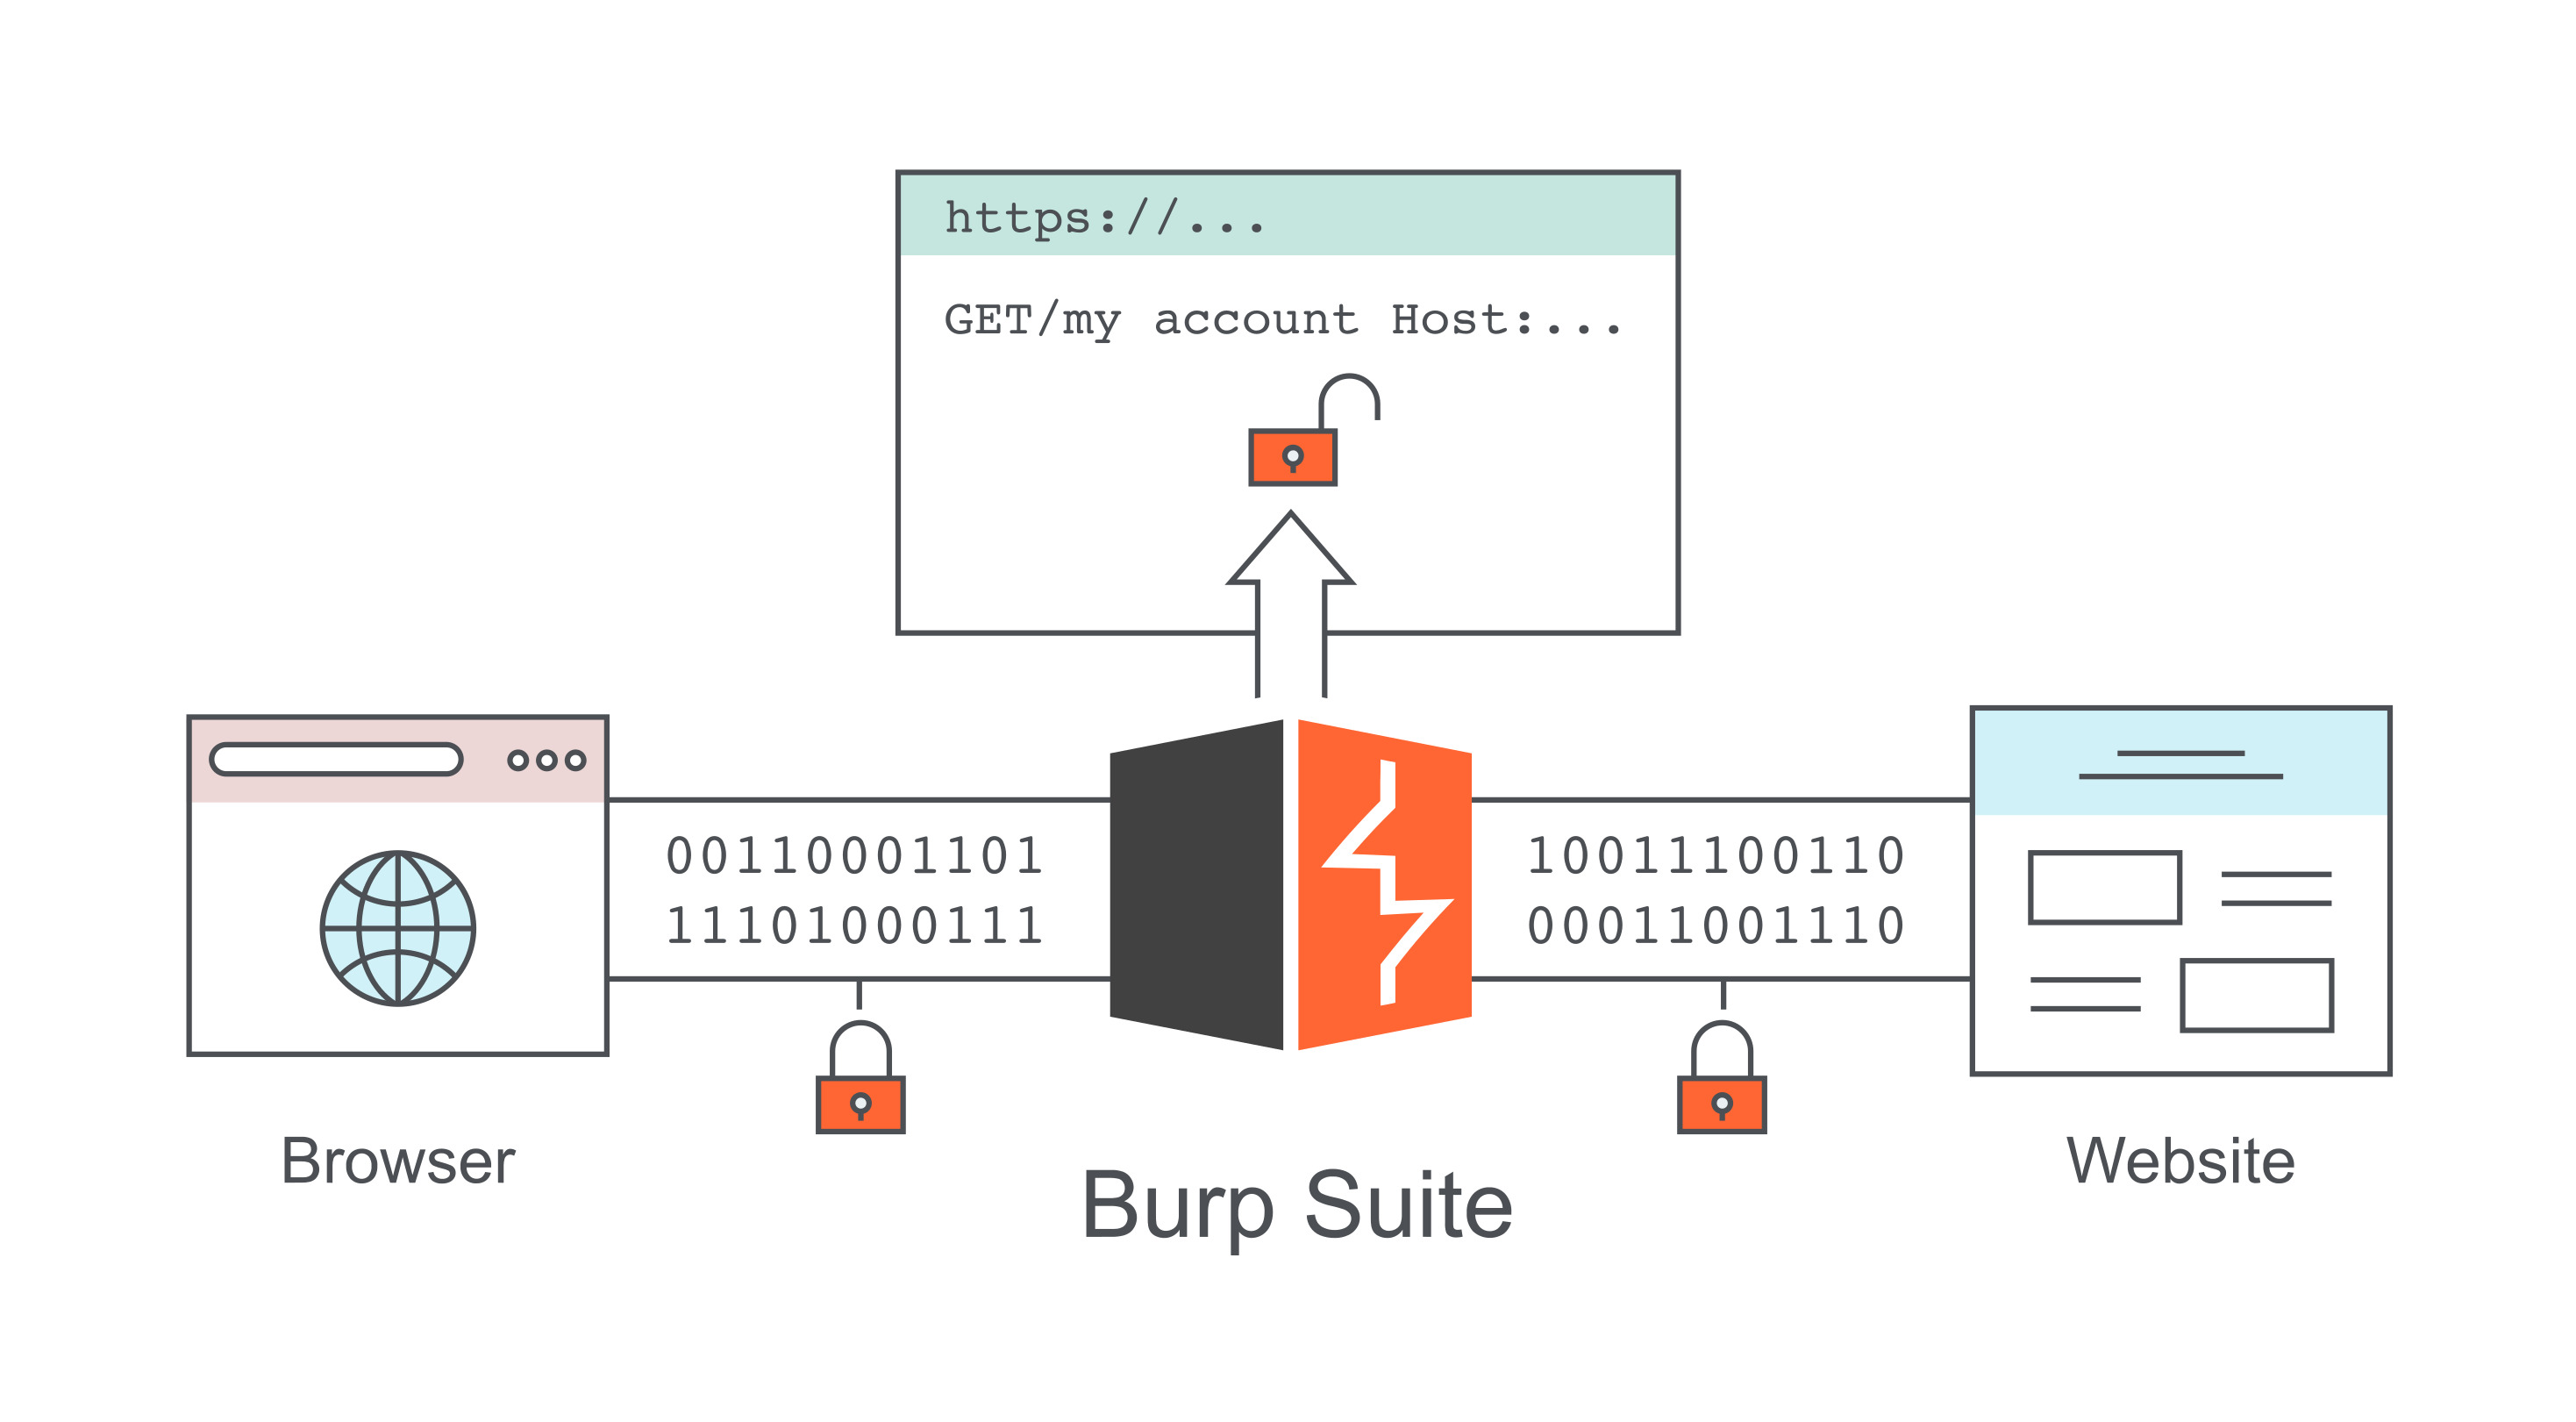
\includegraphics[width=0.9\textwidth]{Images/proxy.jpg}
        \label{fig:Burp-Proxy-img}
    \end{figure}
%----------------------------------------------------------------------------------------
%	Key Features - Scanner
%----------------------------------------------------------------------------------------     
\item \textbf{Scanner}
    \begin{fullwidth}
        Automatically scan web applications for common security vulnerabilities such as SQL injection, cross-site scripting (XSS), and more. It can also crawl a website to discover and map its structure and content
    \end{fullwidth}
    
    \begin{figure}[H]            
        \centering
        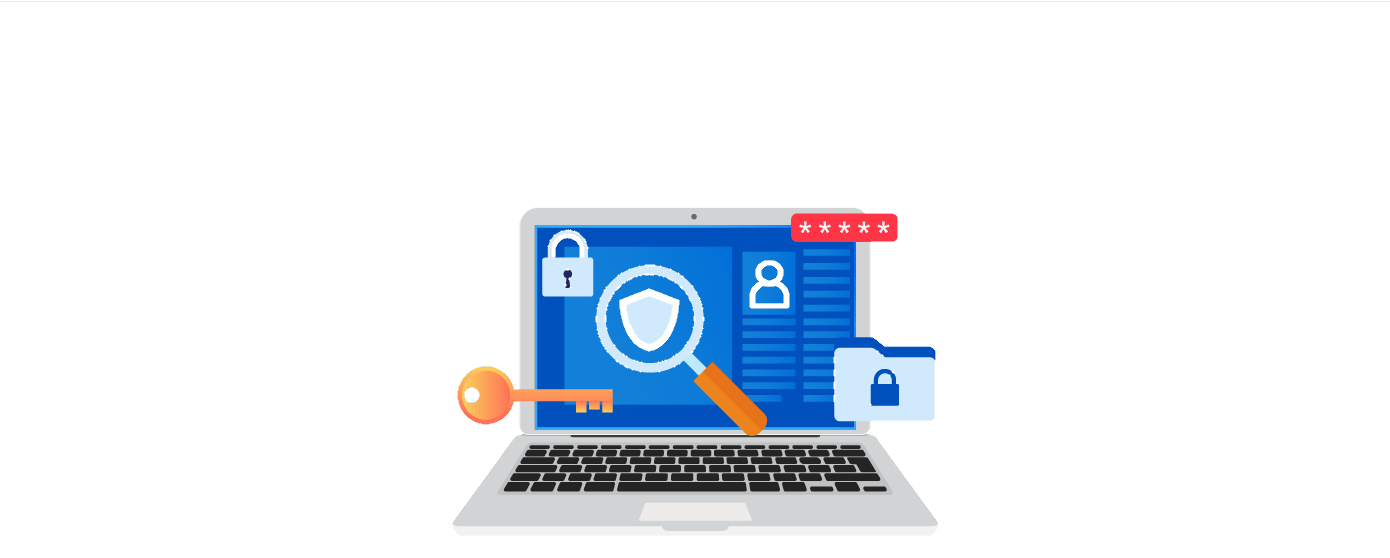
\includegraphics[width=1\textwidth]{scanner-trans.png}                
        \label{fig:enter-label}
    \end{figure}

%----------------------------------------------------------------------------------------
%	Key Features - Intruder
%---------------------------------------------------------------------------------------- 
\item \textbf{Intruder}
\begin{fullwidth}
    Burp Intruder is a tool for automating customized attacks against web applications. It en-

ables you to configure attacks that send the same HTTP request over and over again, in-

serting different payloads into predefined positions each time.
\end{fullwidth}

7 of 16



%----------------------------------------------------------------------------------------
%	Key Features - Repeater
%----------------------------------------------------------------------------------------
\item \textbf{Repeater}
\begin{fullwidth}
   It is used to  manually manipulate and re-send requests to test how the application responds to different inputs. Burp Repeater used to send a request of interest over and over again. This let us to study the target website's response to different input without having to intercept the request each time.
  \begin{figure}[H]
      \centering
      
\includegraphics[width=0.25\linewidth]{rsz_repeater-trans.png}
  \end{figure}
\end{fullwidth}
\end{itemize}

%----------------------------------------------------------------------------------------
%	Getting Started
%----------------------------------------------------------------------------------------
\addcontentsline{toc}{section}{Getting Started}
\section*{Getting Started}

\begin{fullwidth}
    Let's look at Burp Suite installation and usage before diving deeply into how to test a website. We will cover the following subjects in this section: 
\begin{enumerate}
	\item Downloading and installing Burp Suite.
        \item Intercepting HTTP traffic with Burp Proxy.
        \item Modifying requests in Burp Proxy.
        \item Manually reissuing requests with Burp Repeater.
        \item Automatically test on payloads with Burp Intruder.
        \item Running your first scan.
\end{enumerate}
\end{fullwidth}

%----------------------------------------------------------------------------------------
%	Getting Started - Download & Install
%----------------------------------------------------------------------------------------
\addcontentsline{toc}{subsection}{Download and install}
\subsection*{Download and install}

\subsubsection*{Step 1: Download}
\begin{fullwidth}
    Use the links below to download the latest version of Burp Suite \textbf{Professional} or \textbf{Community} Edition.

\begin{center}
    \href{https://portswigger.net/burp/releases/professional-community-2023-9-4?requestededition=professional&requestedplatform=}{\color{orange}Professional Edition\faIcon{link}} 
\qquad
\href{https://portswigger.net/burp/releases/professional-community-2023-9-4?requestededition=community&requestedplatform=}{\color{orange}Community Edition\faIcon{link}} 
\end{center}


Though Professional version is paid, you can apply for free trial ---{Anika fill these} ---.

\end{fullwidth}


\subsubsection*{Step 1: Install}

Just run the \textbf{installer} downloaded.


%----------------------------------------------------------------------------------------
%	Getting Started - Intercepting HTTP Request
%----------------------------------------------------------------------------------------
\addcontentsline{toc}{subsection}{Intercepting HTTP traffic}
\subsection*{Intercepting HTTP traffic with Burp Proxy.}
\begin{fullwidth}
    to use proxy, open burp suite. Go to proxy tab. Make sure that intercept is turned off and go to http history and study the incoming and outgoing data traffic.
\end{fullwidth}
\begin{figure}[H]
    \centering
    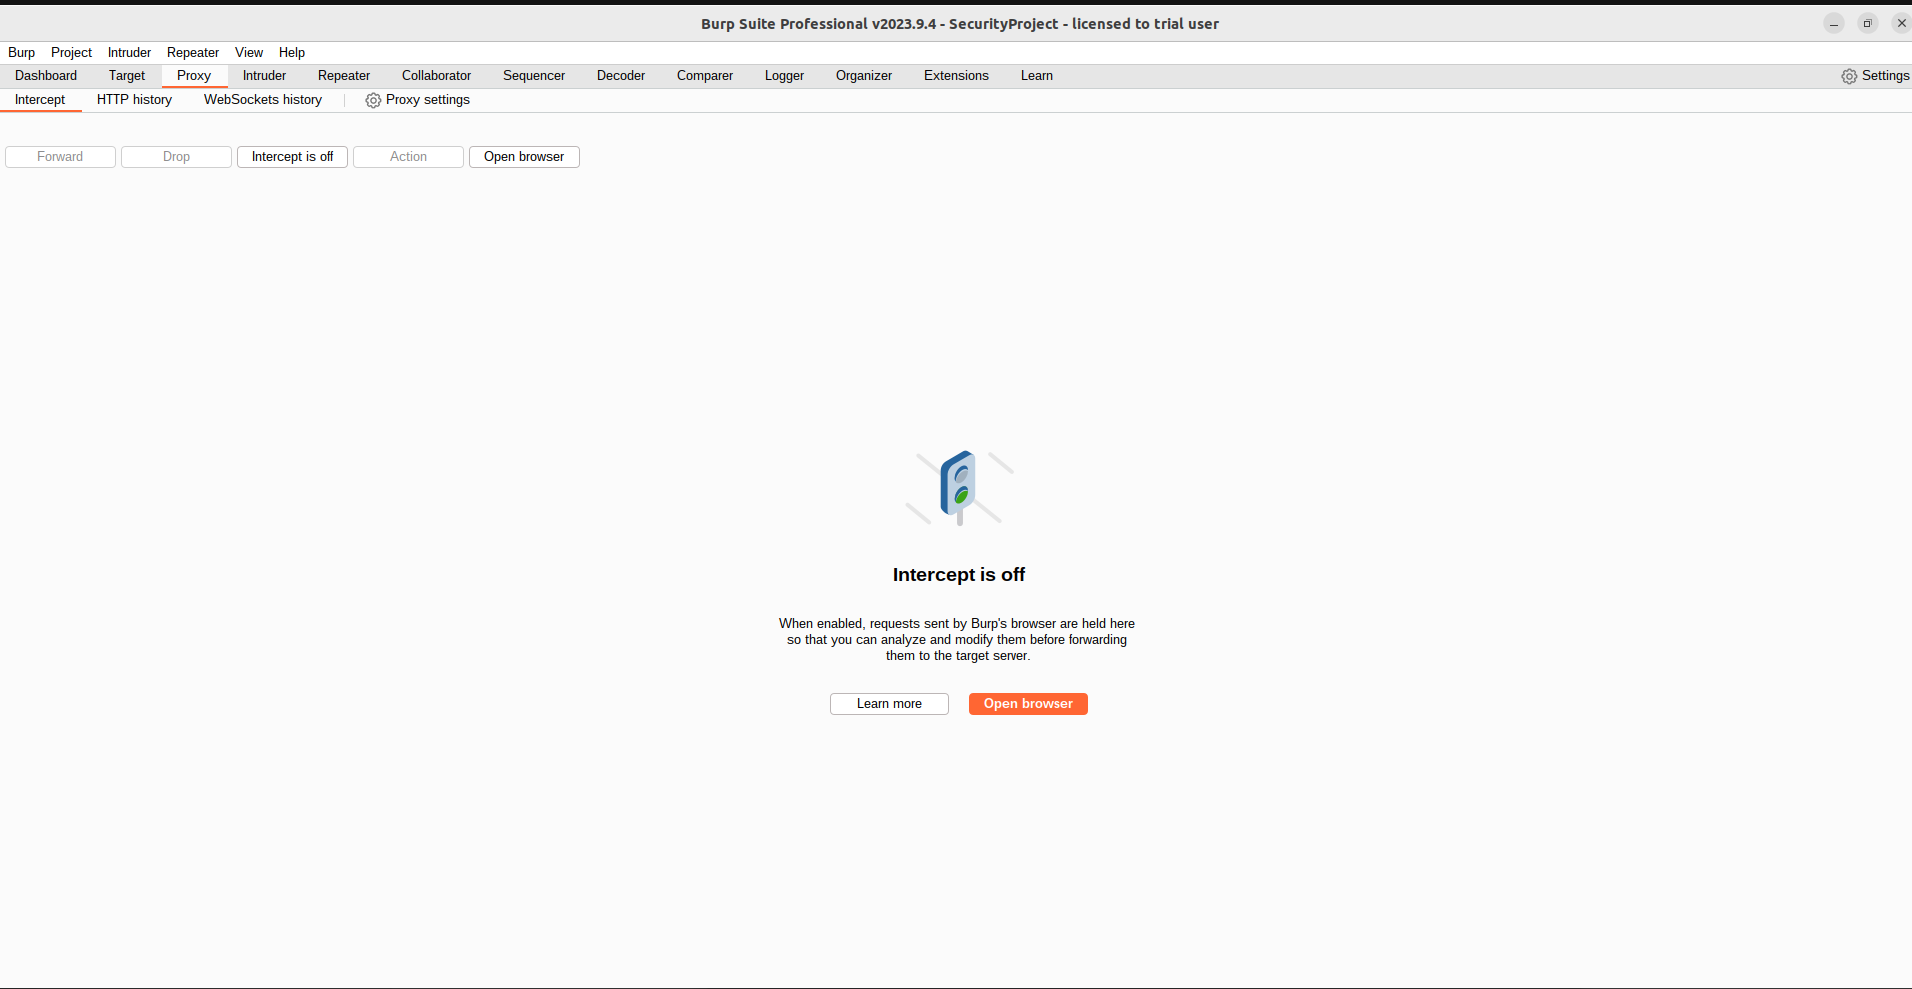
\includegraphics[width=1\textwidth]{Images/anikaScreensots/Proxy1.png}
    \caption{go to proxy tab}
    \label{fig:enter-label}
\end{figure}

\begin{figure}[H]
    \centering
    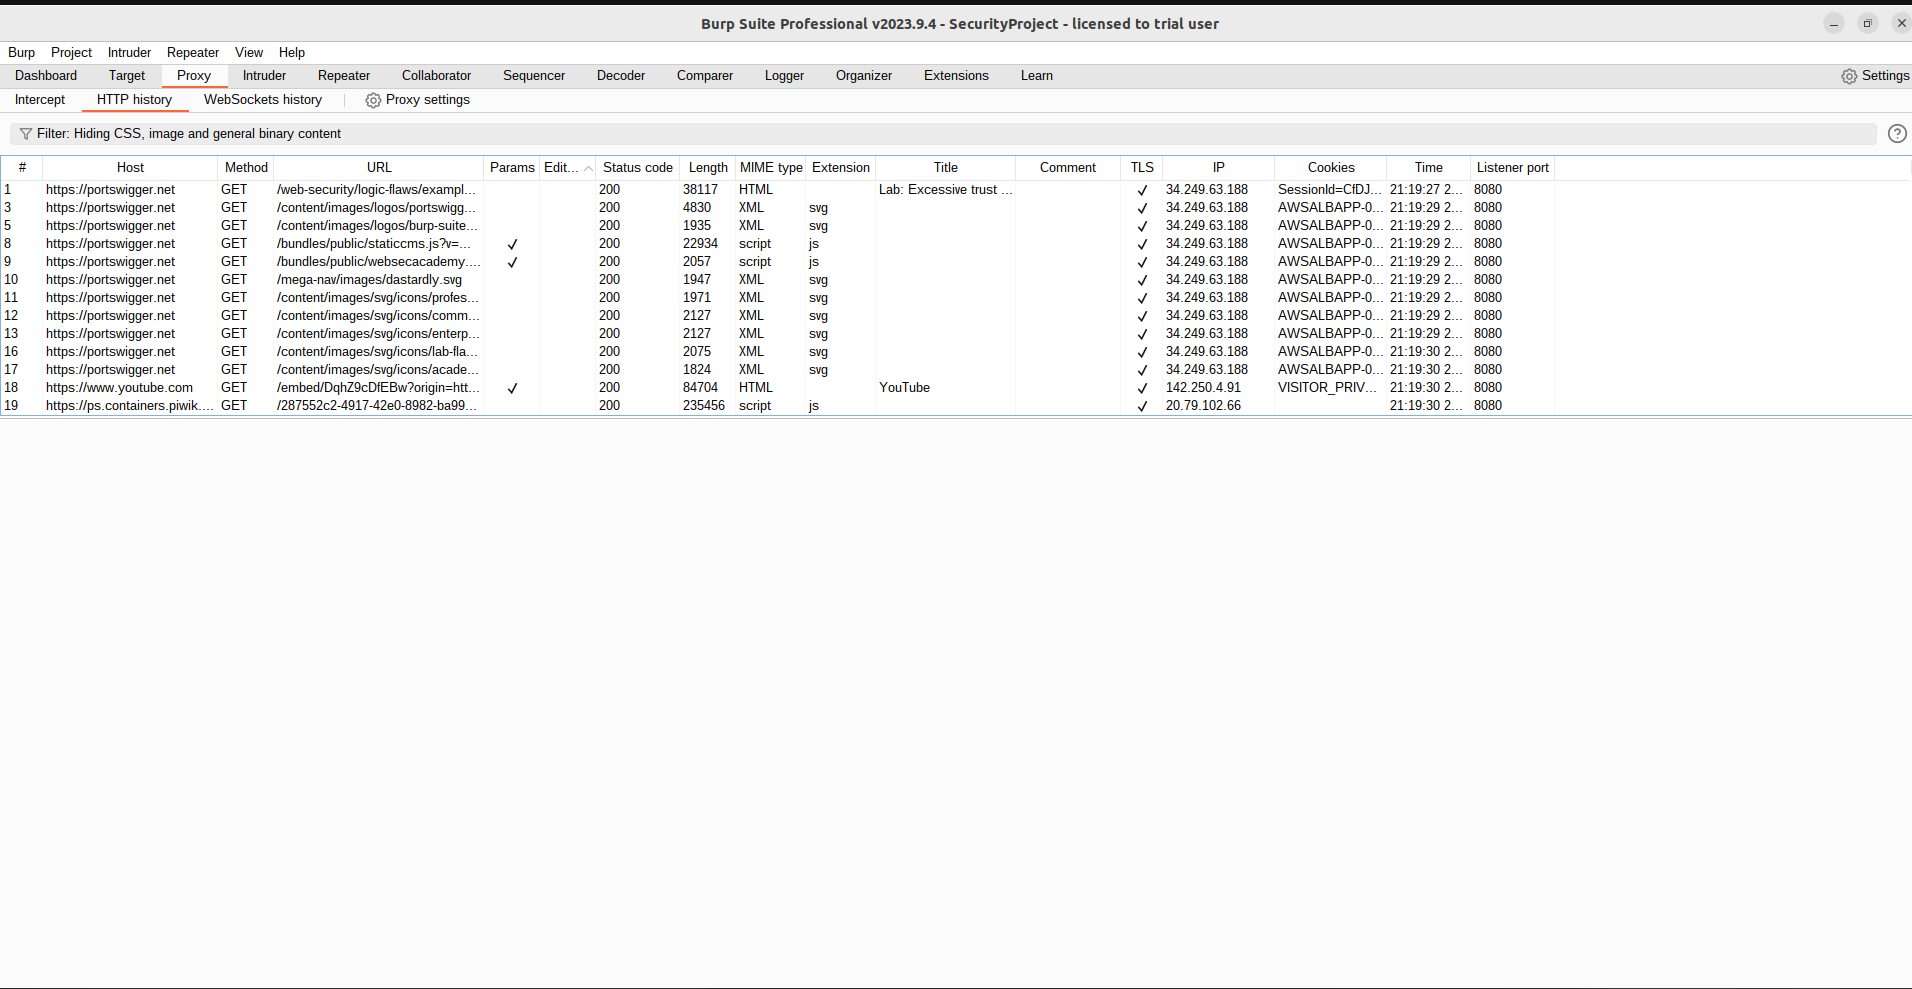
\includegraphics[width=1\textwidth]{Images/anikaScreensots/proxy2.png}
    \caption{examine http history}
    \label{fig:enter-label}
\end{figure}
examine each request in details by by clicking on a request

\begin{figure}[H]
    \centering
    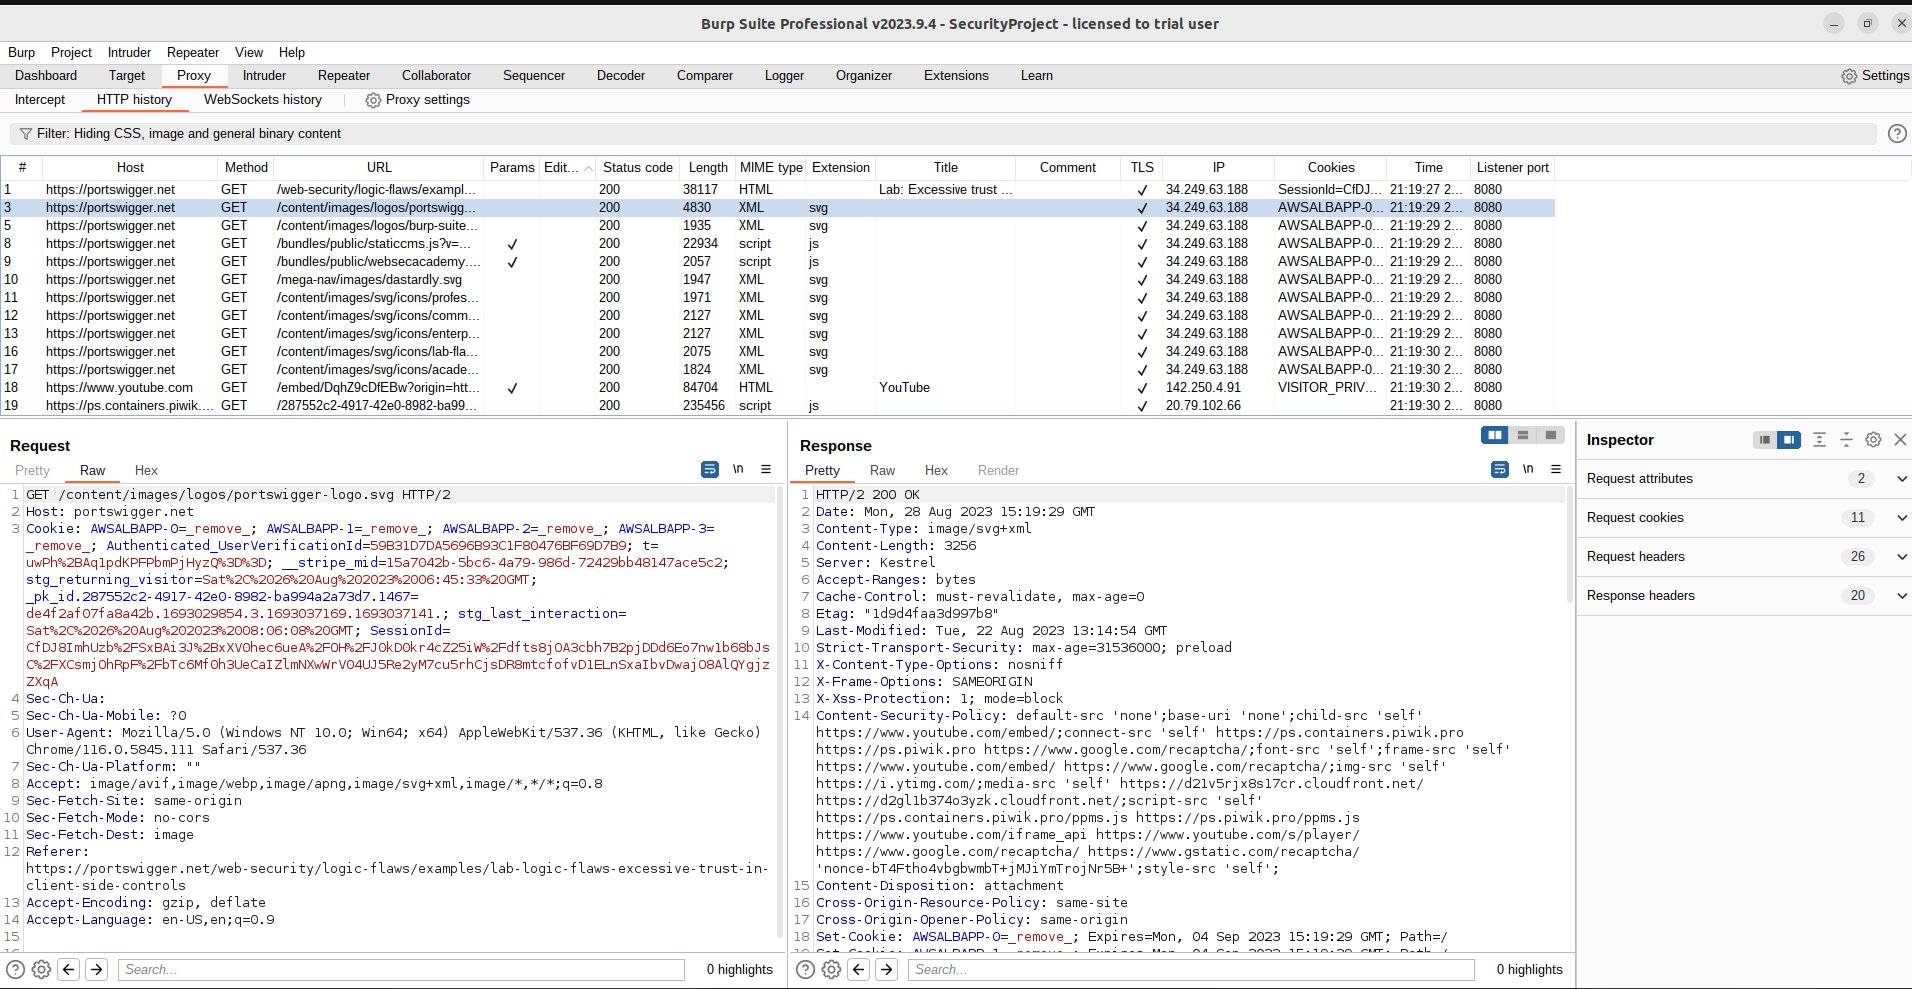
\includegraphics[width=1\textwidth]{Images/anikaScreensots/proxy3.png}
    \caption{examine request}
    \label{fig:enter-label}
\end{figure}
%----------------------------------------------------------------------------------------
%	Getting Started - Modifying Request
%----------------------------------------------------------------------------------------
\addcontentsline{toc}{subsection}{Modifying Request}
\subsection*{Modifying Request in Burp Proxy.}
\begin{fullwidth}
    Burp Proxy lets you intercept HTTP requests and responses sent between Burp's browser and the target server. This enables you to study how the website behaves when you perform different actions. Then we can intercept that request and modify it any way we went
\end{fullwidth}
\subsubsection*{Steps}
\begin{fullwidth}
    

We will use an website that's vulnerable. First we will go the website, add the item we want to buy on cart

\begin{figure}[H]
    \centering
    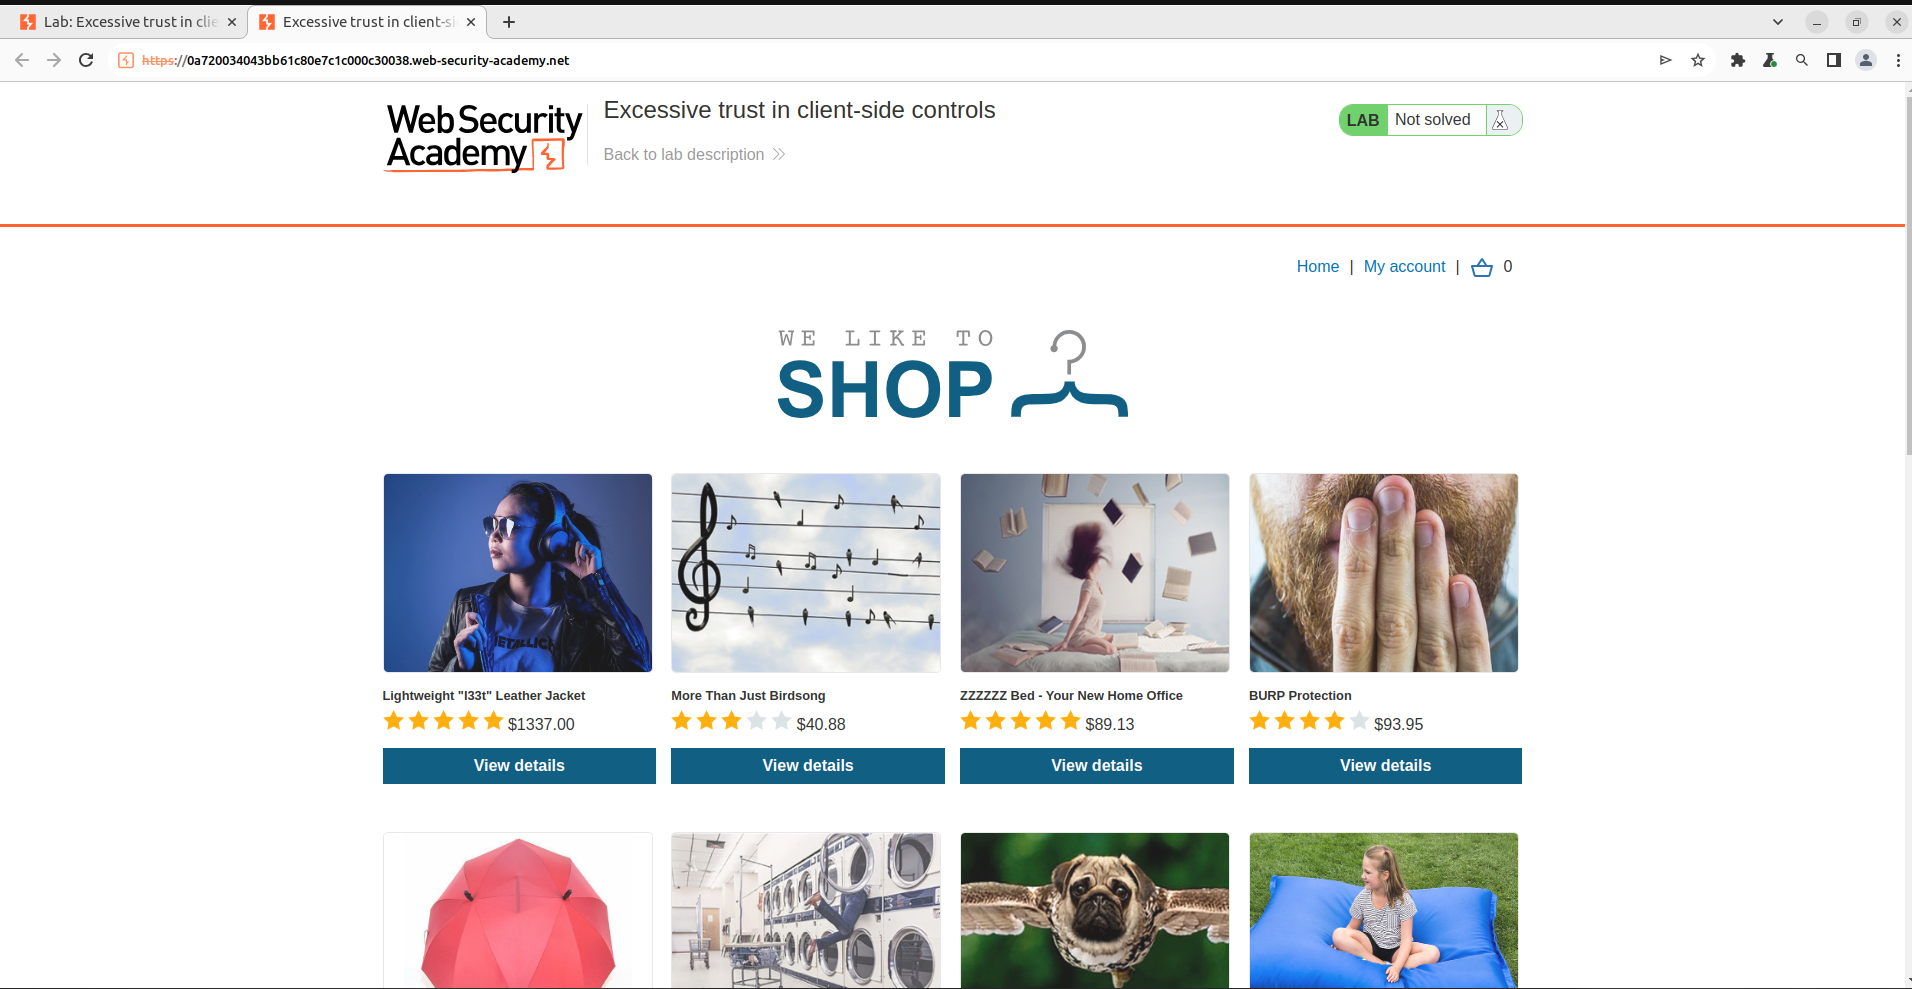
\includegraphics[width=1\textwidth]{Images/anikaScreensots/lab1.png}

\end{figure}

\begin{figure}[H]
    \centering
    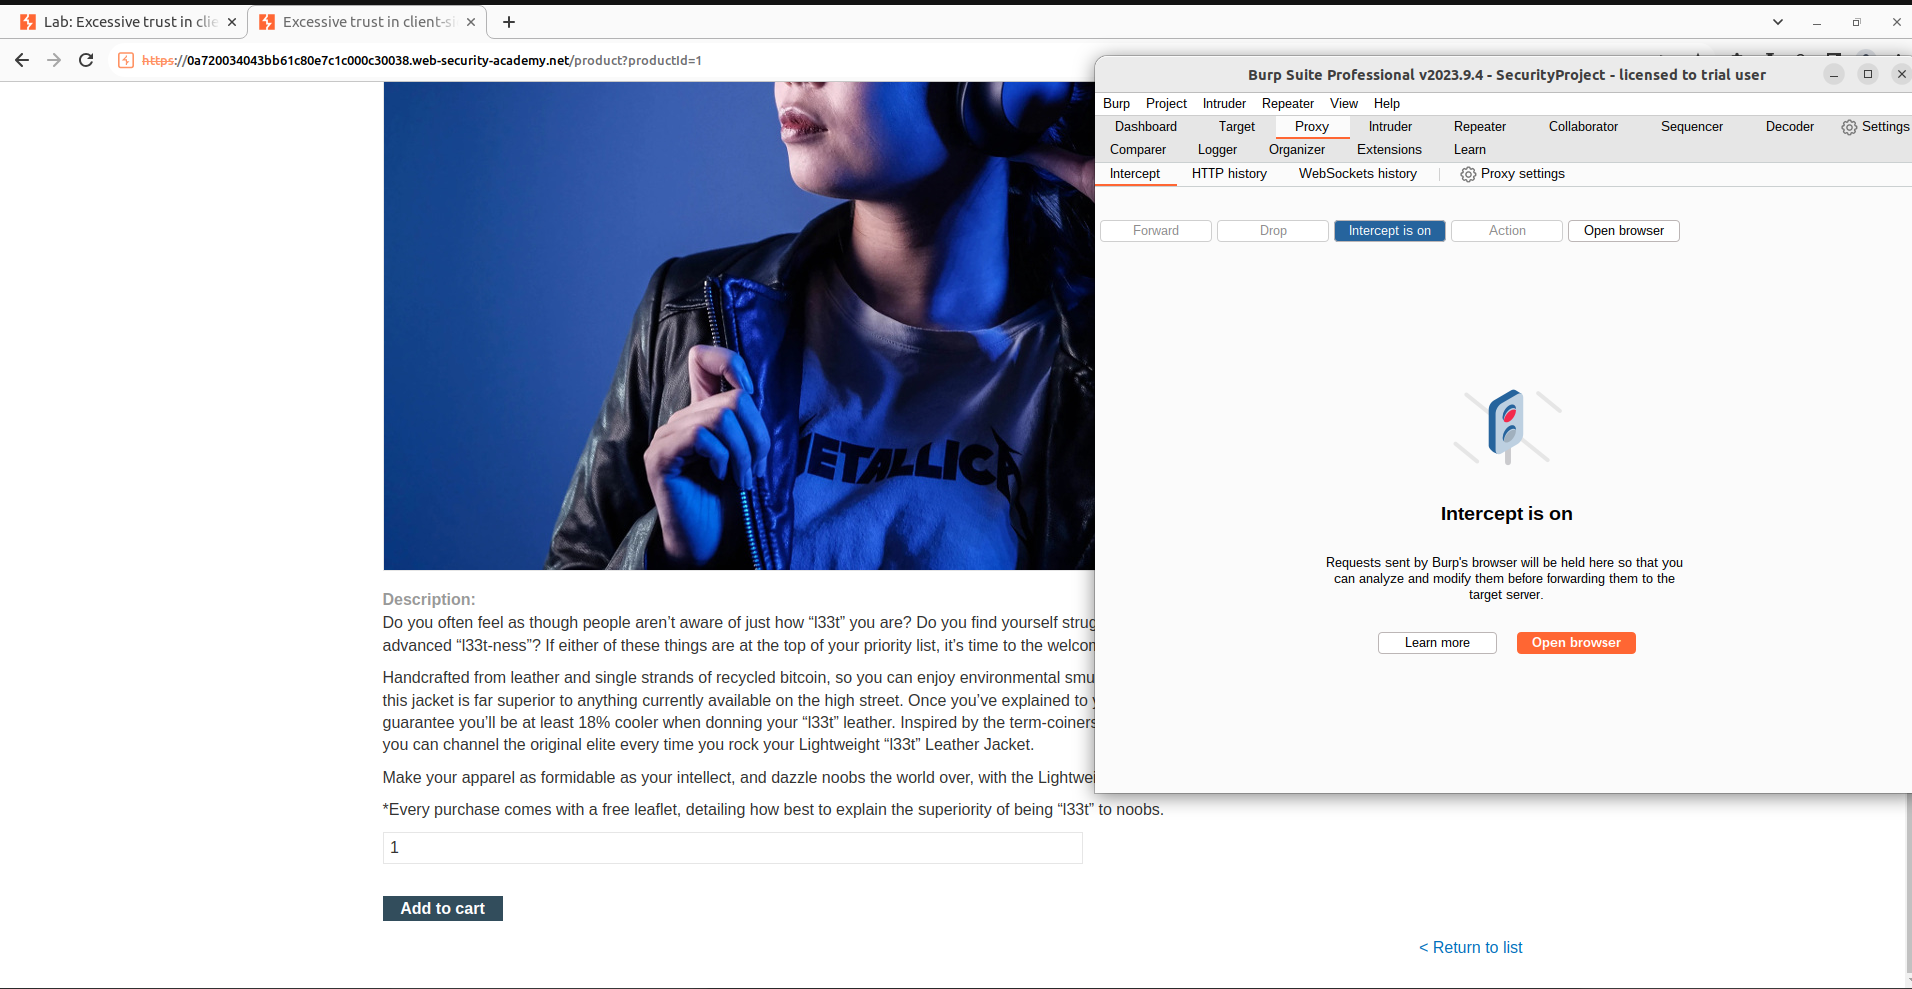
\includegraphics[width=1\textwidth]{Images/anikaScreensots/lab2.png}

\end{figure}

we will turn intercept on before clicking on adding to cart and then examine the intercepted request in burp suite.

\begin{figure}[H]
    \centering
    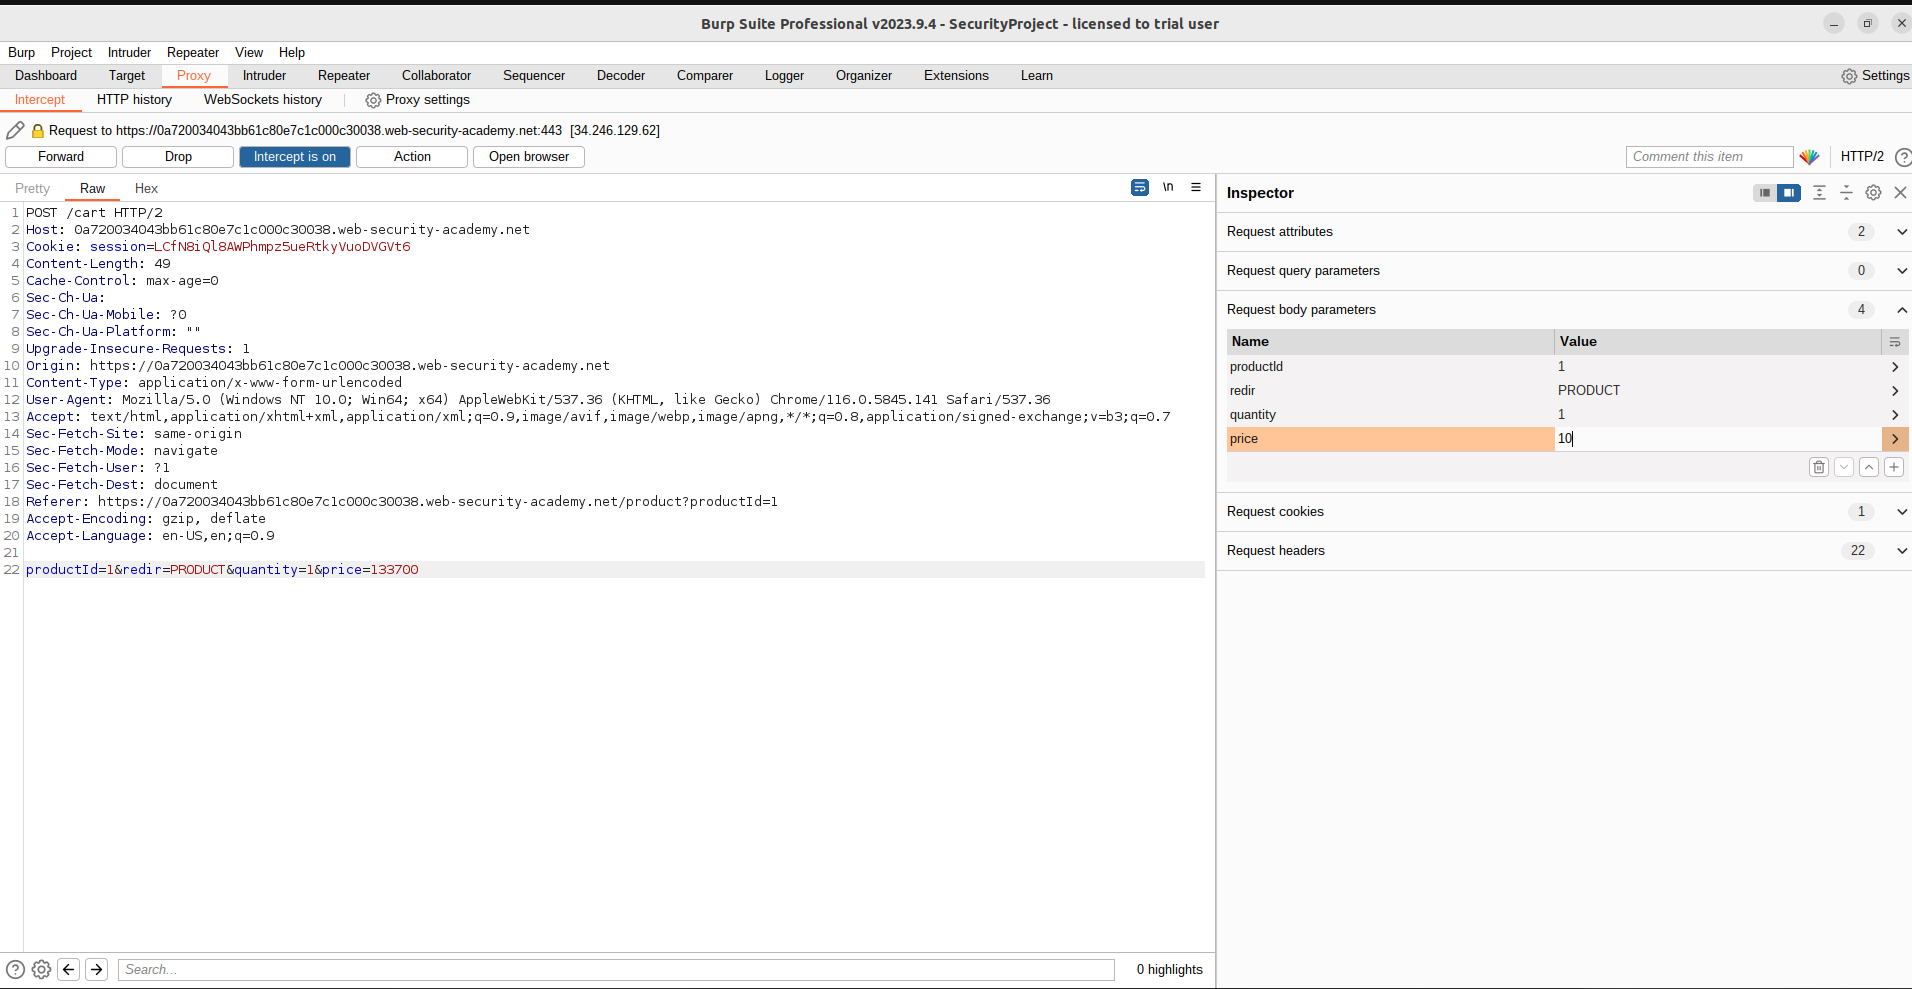
\includegraphics[width=1\textwidth]{Images/anikaScreensots/lab3.png}

\end{figure}
We can see that the price and quantity are right there in the http request and we can modify it to change the price value from high to very very low. And then we will forward that request
\begin{figure}[H]
    \centering
    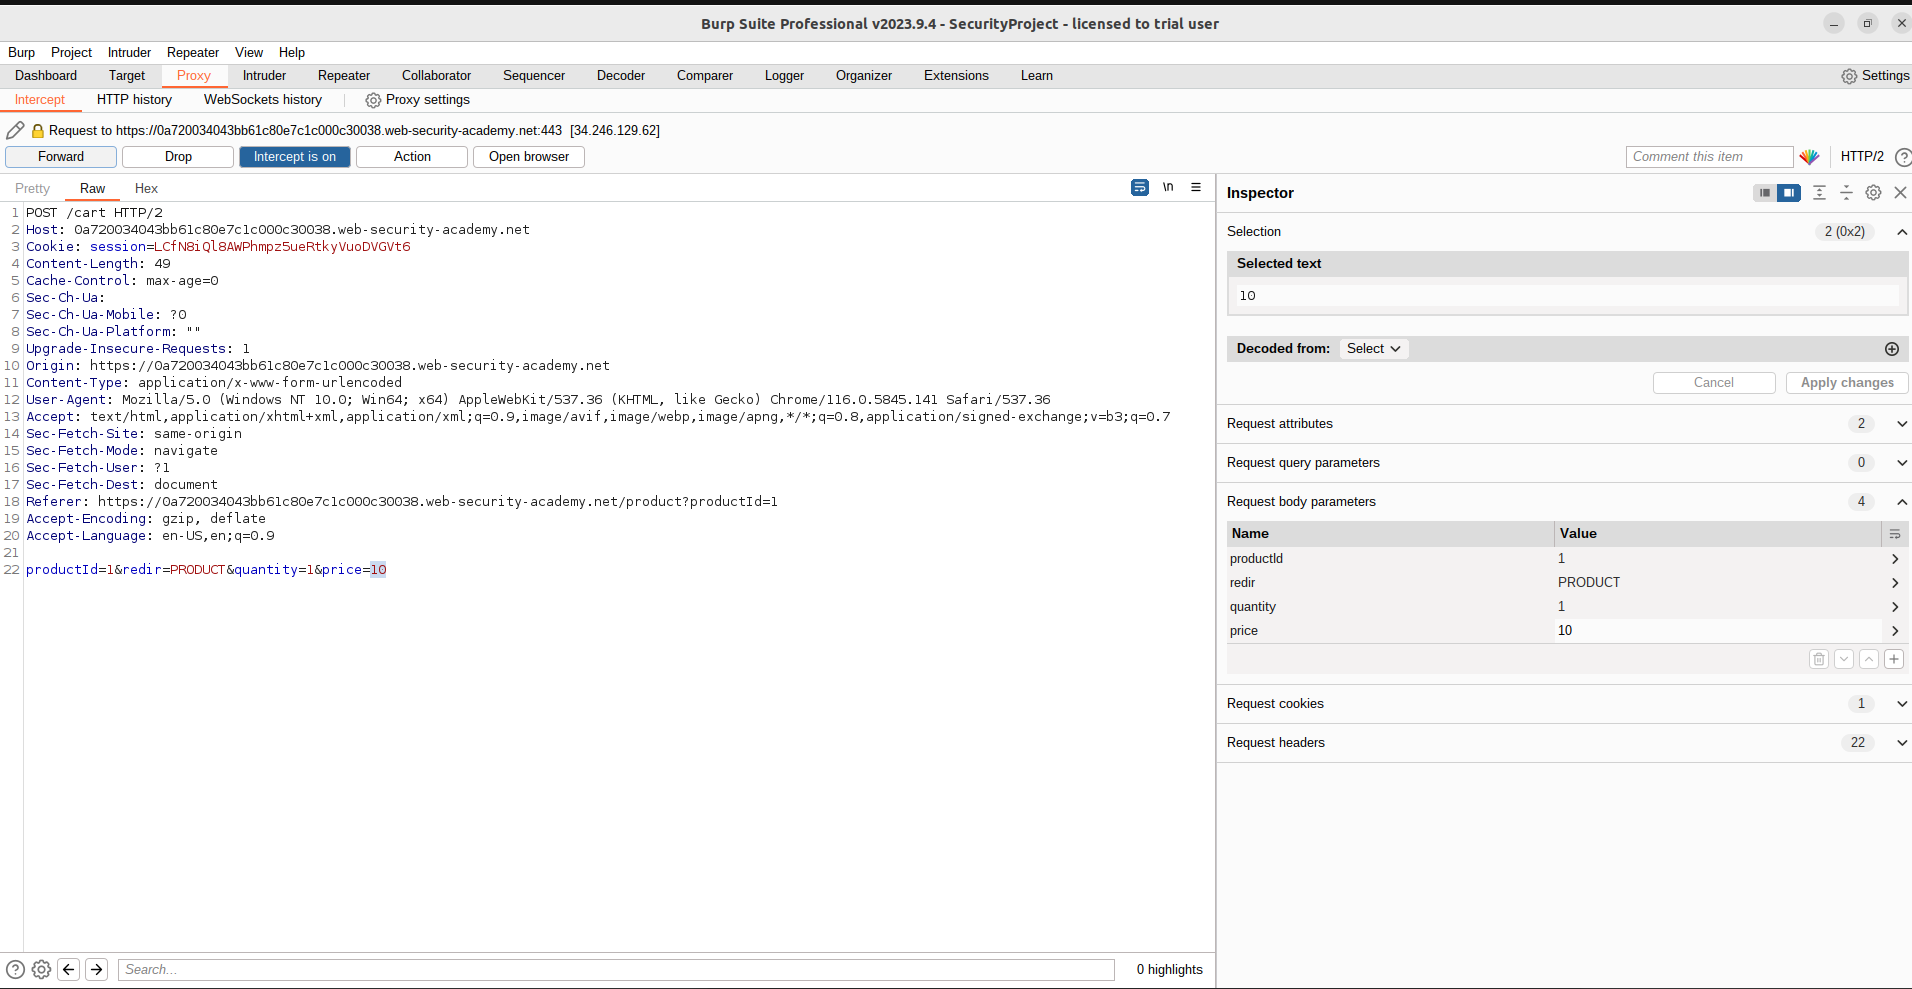
\includegraphics[width=1\textwidth]{Images/anikaScreensots/lab4.png}

\end{figure}

we see that in the cart two items have been added to cart significantly below their actual price.
\begin{figure}[H]
    \centering
    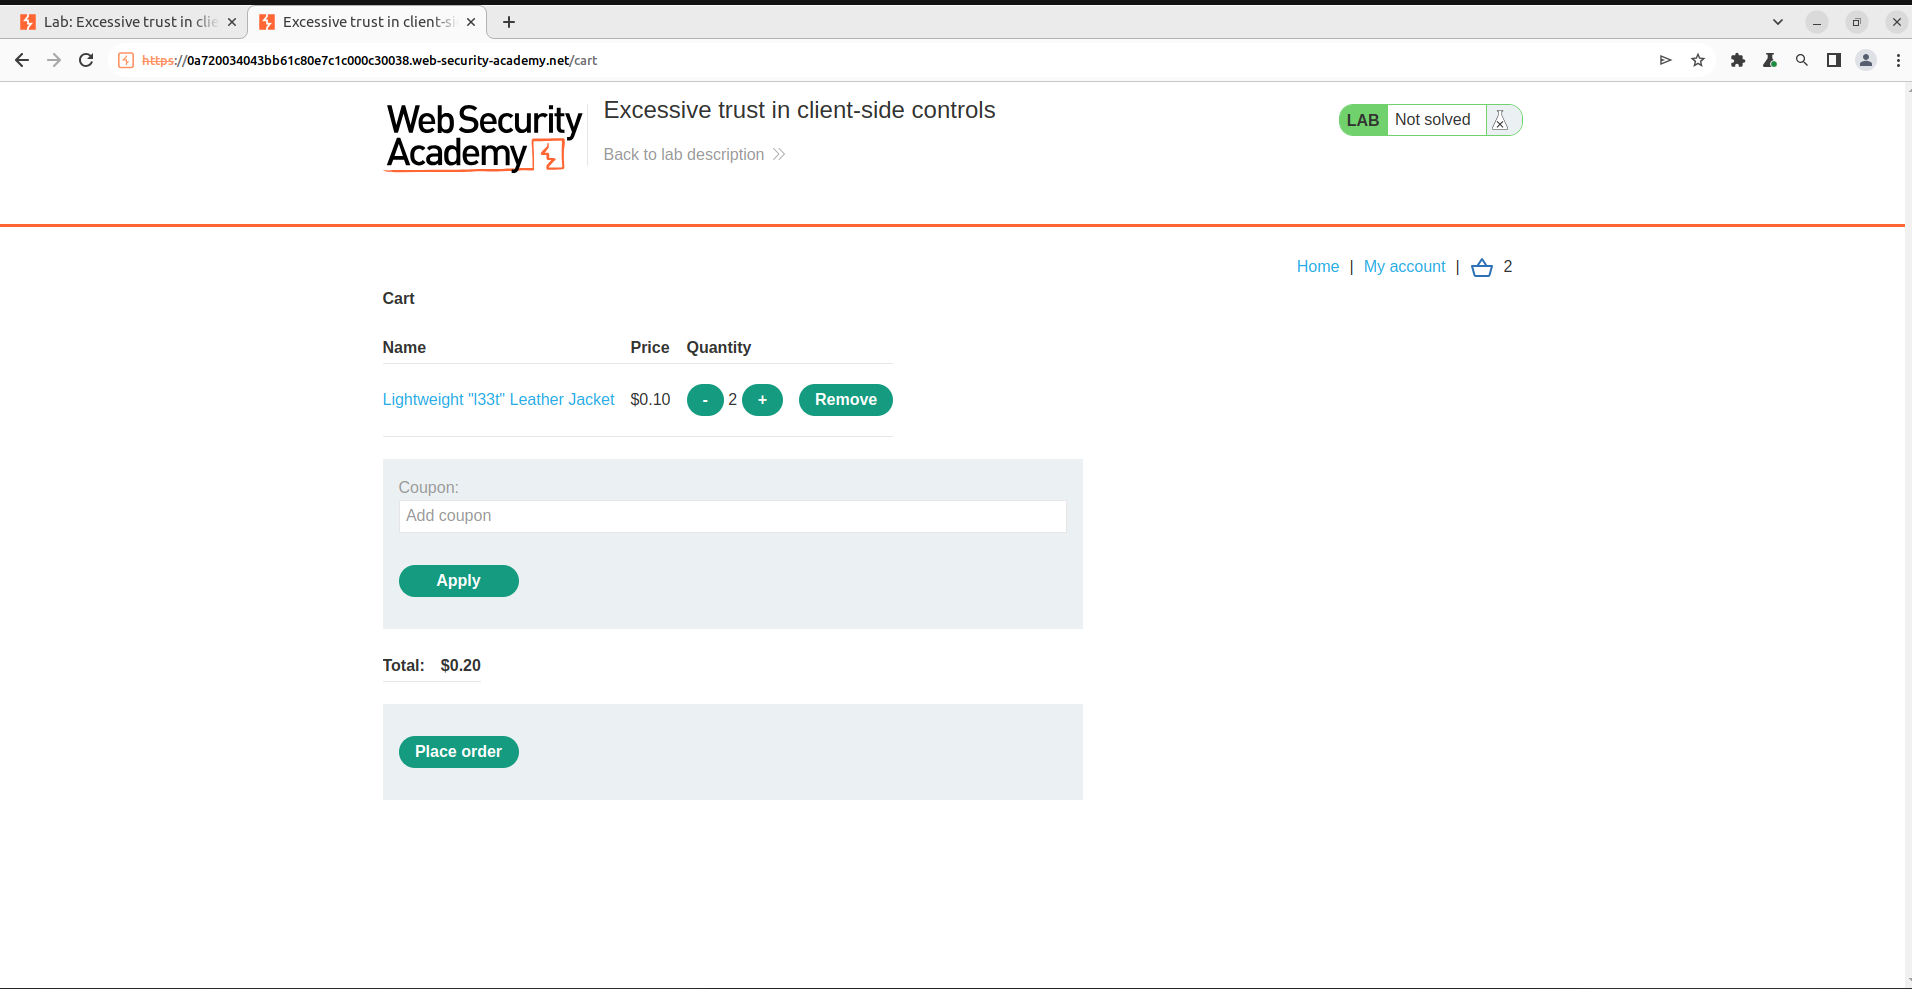
\includegraphics[width=1\textwidth]{Images/anikaScreensots/lab5.png}

\end{figure}
\end{fullwidth}
%----------------------------------------------------------------------------------------
%	Getting Started - Reissuing requests with Burp Repeater
%----------------------------------------------------------------------------------------
\addcontentsline{toc}{subsection}{Reissuing requests}
\subsection*{Reissuing requests with Burp Repeater}
\subsubsection*{Step 1: Identify an interesting request}
\begin{fullwidth}
    Go to {\color{orange}\textbf{Proxy}} > {\color{orange}\textbf{HTTP history}}. Choose a request of interest from the list. And select \textbf{Send to Repeater}
    \begin{figure}[H]
        \centering
        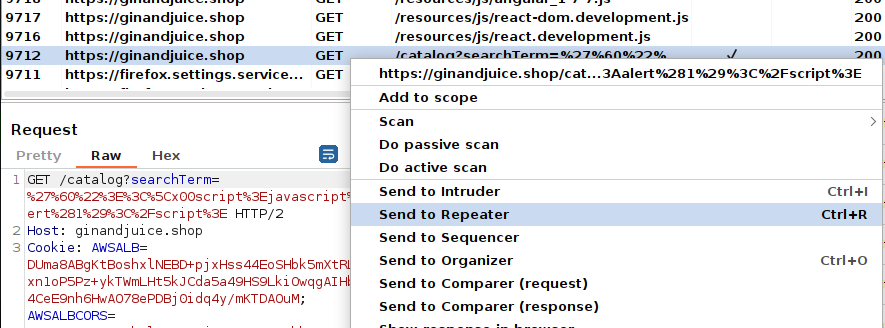
\includegraphics[width=1\linewidth]{Images//using repeater/select_request.png}         
    \end{figure}
\end{fullwidth}


\subsubsection*{Step 2: Explore the request}
\begin{fullwidth}
    Change in any place of interest and click {\color{orange}\textbf{Send}}. Observe the request for any change you made.
    \begin{figure}[H]
        \centering
        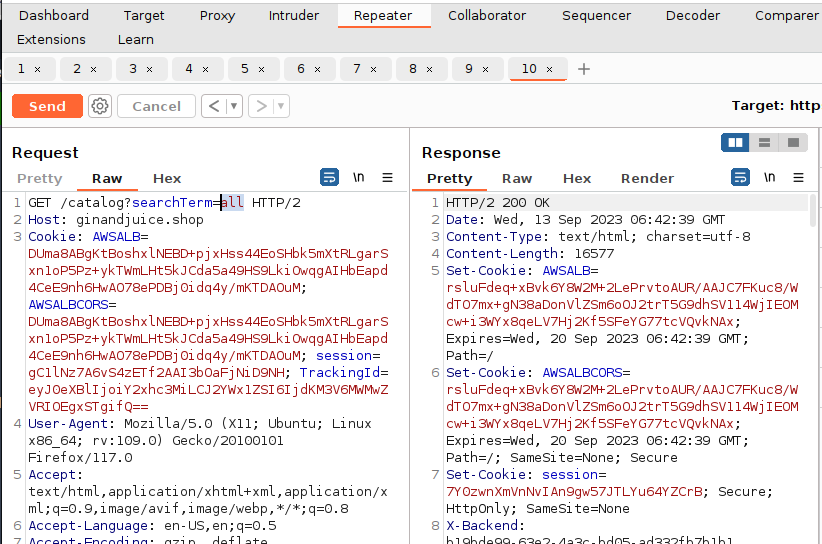
\includegraphics[width=1\linewidth]{Images//using repeater/repeater_window.png}
    \end{figure}
\end{fullwidth}


%----------------------------------------------------------------------------------------
%	Getting Started - Running your first scan.
%----------------------------------------------------------------------------------------
\addcontentsline{toc}{subsection}{Running your first scan}
\subsection*{Running your first scan.}
\subsubsection*{Step 1: Open the Scan Launcher}
\begin{fullwidth}
Go to the {\color{orange}\textbf{Dashboard}} tab and select  {\color{orange}\textbf{New Scan}}.
\begin{figure}[H]
    \centering
    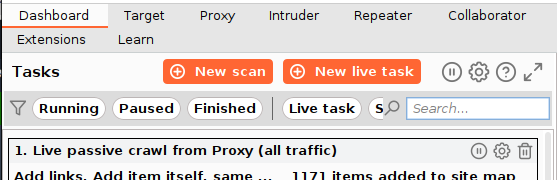
\includegraphics[width=1\linewidth]{Images//using scanner/dashboard_newScan.png}

\end{figure}
\end{fullwidth}

\subsubsection*{Step 2: Enter the URL of the target site}
\begin{fullwidth}
Let’s say, we want to scan the site \href{https://ginandjuice.shop}{\color{orange}gin\&juice.shop}
\begin{figure}[H]
    \centering
    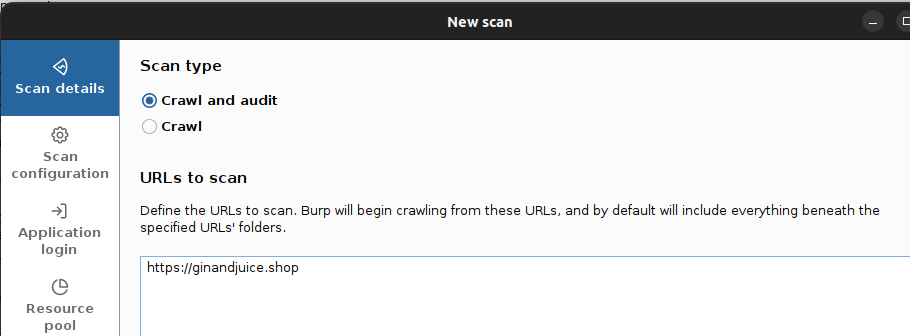
\includegraphics[width=1\linewidth]{Images//using scanner/setting_site.png}

\end{figure}

\end{fullwidth}

\subsubsection*{Step 3: Configure the scan}
\begin{fullwidth}
In the \textbf{Scan Configuration} make sure that \textbf{Use a preset scan mode} and select any scan mode of your choice.
\begin{figure}[H]
    \centering
    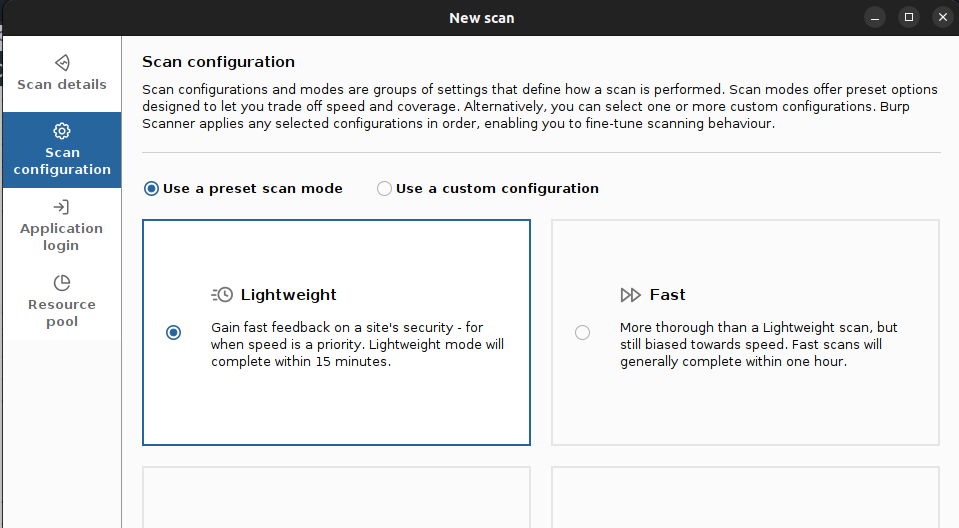
\includegraphics[width=1\linewidth]{Images//using scanner/scan configuration.png}

\end{figure}
\end{fullwidth}

\subsubsection*{Step 4: See the mapping of the site}
\begin{fullwidth}
Go to {\color{orange}\textbf{Target}} > {\color{orange}\textbf{Site map}}. You'll see there is a new entry for \textbf{ginandjuice.shop}. Expand this node to see all of the content that the crawler has managed to discover so far.
\begin{figure}[H]
    \centering
    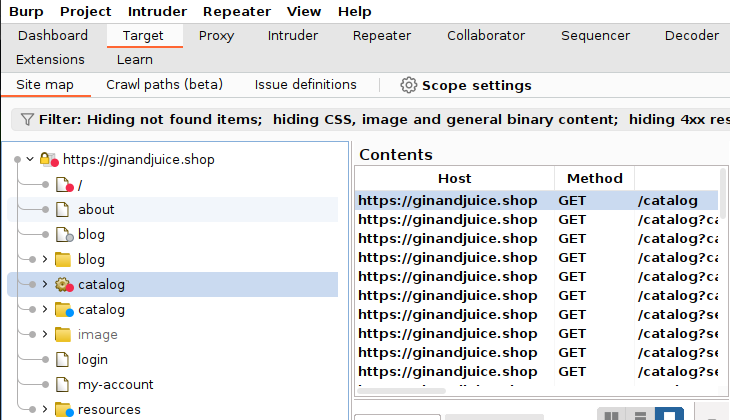
\includegraphics[width=0.5\linewidth]{Images//using scanner/crawled_output.png}

\end{figure}
\end{fullwidth}

\subsubsection*{Step 5: View the identified issues}
\begin{fullwidth}
In the {\color{orange}\textbf{Target}} > {\color{orange}\textbf{Site map}} > {\color{orange}\textbf{Issues}}, you'll see the issue found while scanning the site. If you select an issue it'll indicate where the issue were found and also gives details of that issue below.
\begin{figure}[H]
    \centering
    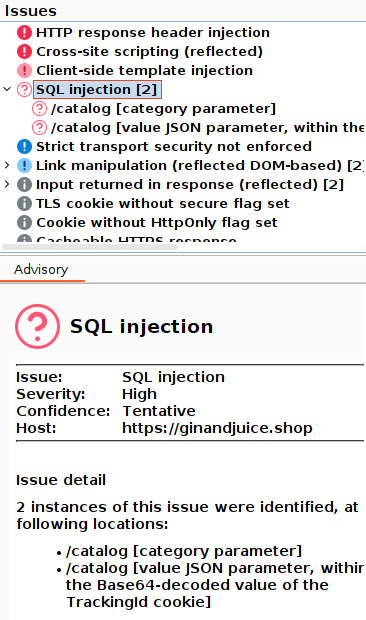
\includegraphics[width=0.75\linewidth]{Images//using scanner/issue.png}

\end{figure}
\end{fullwidth}


%----------------------------------------------------------------------------------------
%	Penetration testing workflow
%----------------------------------------------------------------------------------------
\addcontentsline{toc}{section}{Penetration testing workflow}
\section*{Penetration testing workflow}

\begin{fullwidth}
    Penetration testing with Burp Suite involves a structured workflow to identify and exploit vulnerabilities in web applications. You can use Burp's automated and manual tools to obtain detailed information about your target applications. Below is a step-by-step guide to the typical penetration testing process using Burp Suite:
\end{fullwidth}

\begin{enumerate}

    \item Setting Test Scope \nonumsidenote{Note : \newline {\scriptsize There are many other ways to test an website. But here we cover only these stages. To explore more, you can visit : \newline \href{https://portswigger.net/burp/documentation/desktop/testing-workflow}{\color{orange}Testing-Workflow\faIcon{link} } }
}
    \item Map the target application
    \item Analyzing the attack surface
    \item Testing authentication mechanisms
    \item Testing session management mechanisms
    \item Testing input validation	
\end{enumerate}



%----------------------------------------------------------------------------------------
%	Penetration testing workflow - Setting Test Scope
%----------------------------------------------------------------------------------------
\addcontentsline{toc}{subsection}{Setting Test Scope}
\subsection*{Stage-1 : Setting Test Scope}
\begin{fullwidth}
    As Burp Suite capture your browsing, so there will be many unnecessary things as we browse. But we only want to focus on our target site. For this we have to Configure Project Scope of Burp Suite.
\newline 
For example, let's use \href{https://ginandjuice.shop}{\color{orange}gin\&juice.shop} as our test scope. Now we have to configure Burp Suite's project scope settings. 


\subsubsection*{Step-1 : Change in Project Scope}
\begin{itemize}
	\item Go to project \textbf{settings}
\begin{figure}[H]
    \centering
    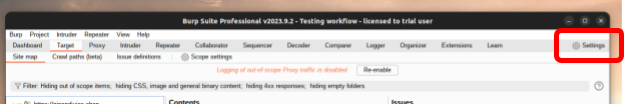
\includegraphics[width=1\linewidth]{Images//Setting Test Scope/settings.png}
    
    
\end{figure}
	\item Go to {\color{orange}\textbf{Project}} > {\color{orange}\textbf{Scope}}
            \begin{itemize}
                \item Here, 2 options will show - \textbf{Include in scope} and \textbf{Exclude in scope.} For our case we did
\begin{figure}[H]
    \centering
    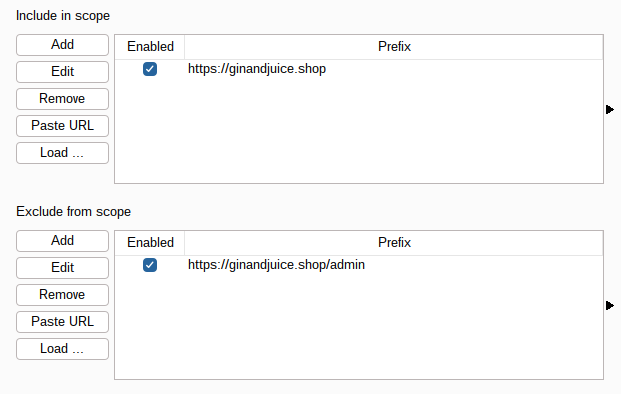
\includegraphics[width=1\linewidth]{Images/Setting Test Scope/scope_site.png}    
\end{figure}
            \end{itemize}	

\end{itemize}


\subsubsection*{Step-2 : Filter out Out-of-Scope capturing}
\begin{itemize}
    \item Then close the Settings tab. And go to the {\color{orange}\textbf{Target}} tab.
    \item There may be other http requests included in that window. You can filter out the unwanted request by 
    \begin{figure}[H]
    \centering
        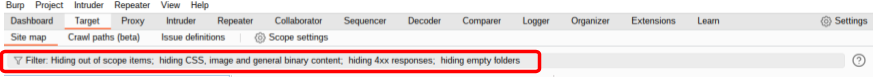
\includegraphics[width=1\linewidth]{Images//Setting Test Scope/filter.png}
    \end{figure}
    \begin{figure}[H]
    \centering
        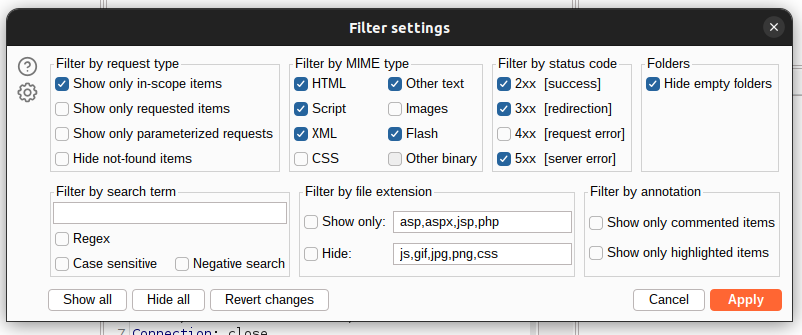
\includegraphics[width=1\linewidth]{Images/Setting Test Scope/filter-2.png}   
    \end{figure} 

\end{itemize}
\end{fullwidth}



%----------------------------------------------------------------------------------------
%	Penetration testing workflow - Mapping the web application
%----------------------------------------------------------------------------------------
\addcontentsline{toc}{subsection}{Mapping the web application}
\subsection*{Stage-2 : Mapping the web application}
\begin{fullwidth}
    The best way to start testing an application is to map its contents. This enables you to understand what the application does and how it behaves. You can then identify interesting areas that you want to probe for vulnerabilities.
    
\subsubsection*{Step-1 : Begin Scan}
\begin{itemize}
    \item If you have done the previous stage, then go to {\color{orange}\textbf{Target}} > {\color{orange}\textbf{Site Map}}. You’ll notice that automatically there is a node created to  represent the target domain.
    \begin{figure}[H]
        \centering
        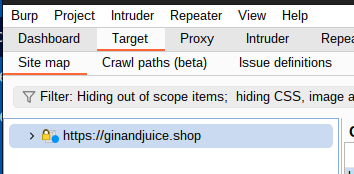
\includegraphics[width=0.5\linewidth]{Images//Mapping/Site Map-1.png}
        
        
    \end{figure}
    
    \item Right-click the root node for the domain, then select Scan. The New scan dialog opens:
        \begin{itemize}
            \item If you have any application login credentials, select Application login and enter the credentials. (In our case we don’t do this)

            \item Under {\color{orange}\textbf{Scan type}}, select {\color{orange}\textbf{Crawl}} or {\color{orange}\textbf{Crawl and Audit}}.

            \item Click OK to start the scan. Burp Scanner crawls the application. Notice that the site map automatically populates as Burp Scanner discovers content
            
        \end{itemize}
\end{itemize}
        \begin{figure}[H]
            \centering
            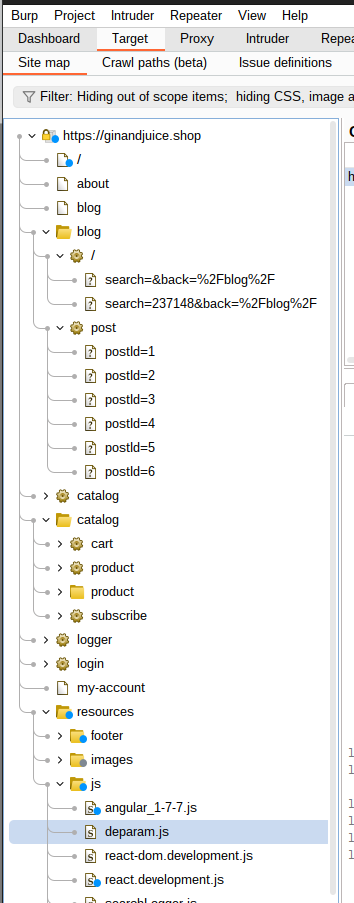
\includegraphics[width=0.5\linewidth]{Images//Mapping/after_scan.png}
            
            
        \end{figure}
\end{fullwidth}


%----------------------------------------------------------------------------------------
%	Penetration testing workflow - Analyzing the attack surface 
%----------------------------------------------------------------------------------------
\addcontentsline{toc}{subsection}{Analyzing the attack surface }
\subsection*{Stage-3 : Analyzing the attack surface }
\begin{fullwidth}
    While you map the application, you should analyze your findings to identify key attack surfaces. You can use this information to plan your approach for auditing the application. Use Target > Site Map to analyze the information that Burp captures about the application.
    \begin{itemize}
        \item Suppose, select any request from the nodes. 
        \begin{figure}[H]
            \centering
            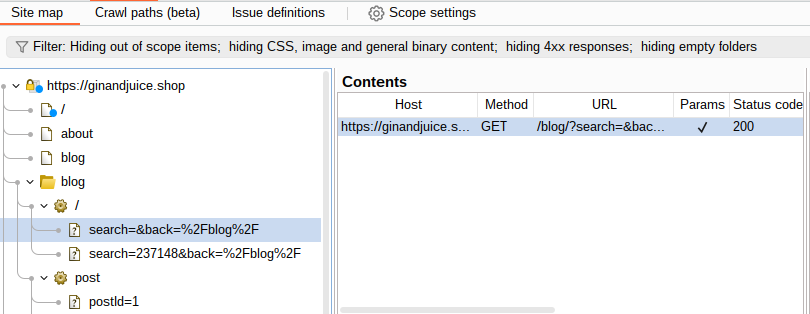
\includegraphics[width=0.5\linewidth]{Images//Mapping/select Request.png}
            
            
        \end{figure}
        \item You can send HTTP messages that you want to investigate further.
        \begin{itemize}
            \item Either by directly sending the request in the browser.
\begin{figure}[H]
    \centering
    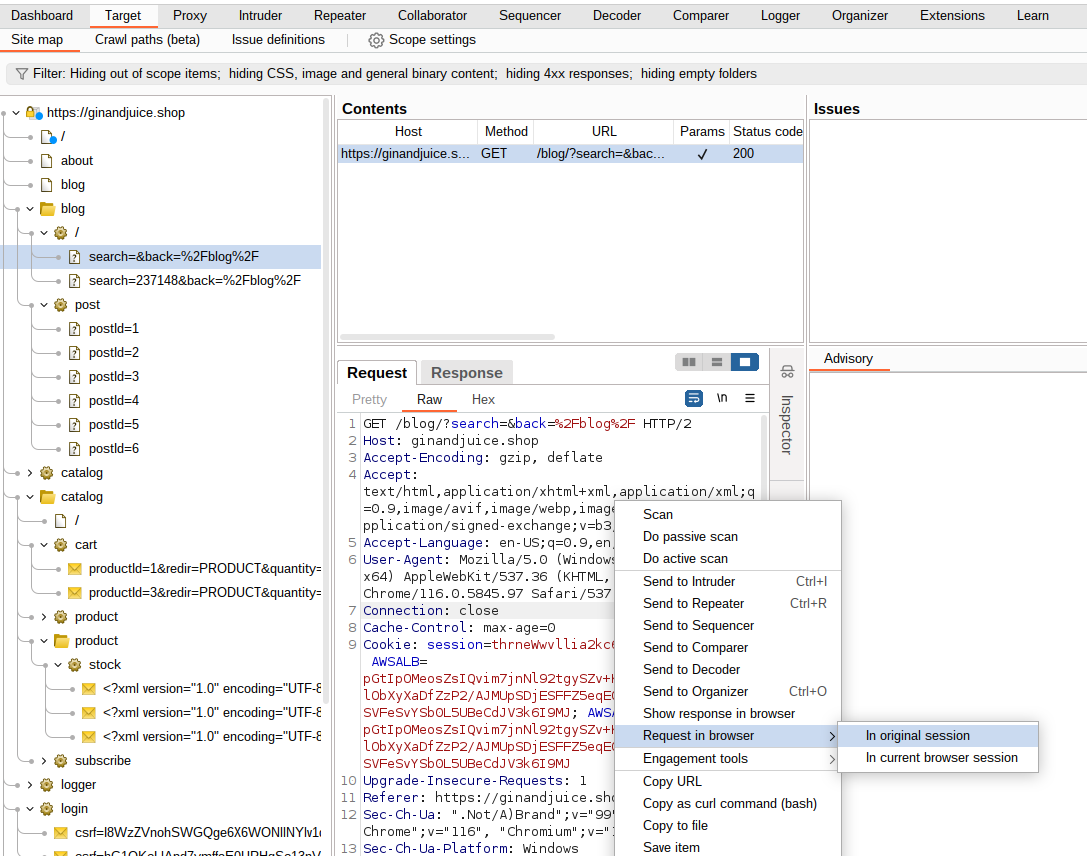
\includegraphics[width=0.5\linewidth]{Images//Mapping/request_browser.png}
    
    
\end{figure}
\begin{figure}[H]
    \centering
    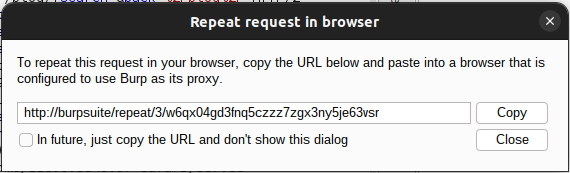
\includegraphics[width=0.5\linewidth]{Images//Mapping/request_browser2.png}
    
    
\end{figure}
            \item Or you can just send the request to the {\color{orange}\textbf{Repeater}}.
        \end{itemize}

    \item You can also use other Burp tools to help you analyze the attack surface and decide where to focus your attention:
        \begin{itemize}
            \item Use Burp Scanner to scan a specific interesting request. Burp Scanner audits only this request. This can flag issues quickly.
            \begin{figure}[H]
                \centering
                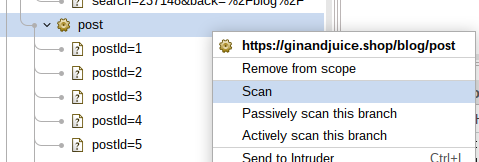
\includegraphics[width=0.5\linewidth]{Images//Mapping/sending_scanner.png}
                
                
            \end{figure}
        \end{itemize}
    \end{itemize}
\end{fullwidth}


%----------------------------------------------------------------------------------------
%	Penetration testing workflow - Testing for vulnerabilities
%----------------------------------------------------------------------------------------
\addcontentsline{toc}{subsection}{Testing for vulnerabilities }
\subsection*{Stage-4 : Testing for vulnerabilities}
\begin{fullwidth}

%----------------------------------------------------------------------------------------
%	Penetration testing workflow - Testing for vulnerabilities - Testing authentication mechanism
%----------------------------------------------------------------------------------------
\addcontentsline{toc}{subsubsection}{Testing authentication mechanism}
\subsubsection*{Testing authentication mechanism}

\begin{fullwidth}Testing authentication mechanisms using Bu rp Intruder is a crucial step in assessing the security of a web application. Authentication is a critical component that safeguards user accounts and sensitive data. Burp Intruder allows security testers to perform various types of attacks to identify vulnerabilities in the authentication process\end{fullwidth}



\subsection*{Enumerating usernames}

\begin{fullwidth}Using burp intruder, we can enumerate a registration or login form. First we will try to login using a random username and password. Then we will examine the request and send it to burp intruder. Burp intruder will keep sending the request with possible different usernames and passwords. We will check the responses to find out any anomaly with one of the inputs in the hope that it might gain us some information \end{fullwidth}


\subsubsection*{Steps}

To test authentication mechanism we will try to login in to a vulnerable website.

\begin{figure}[H]
    \centering
    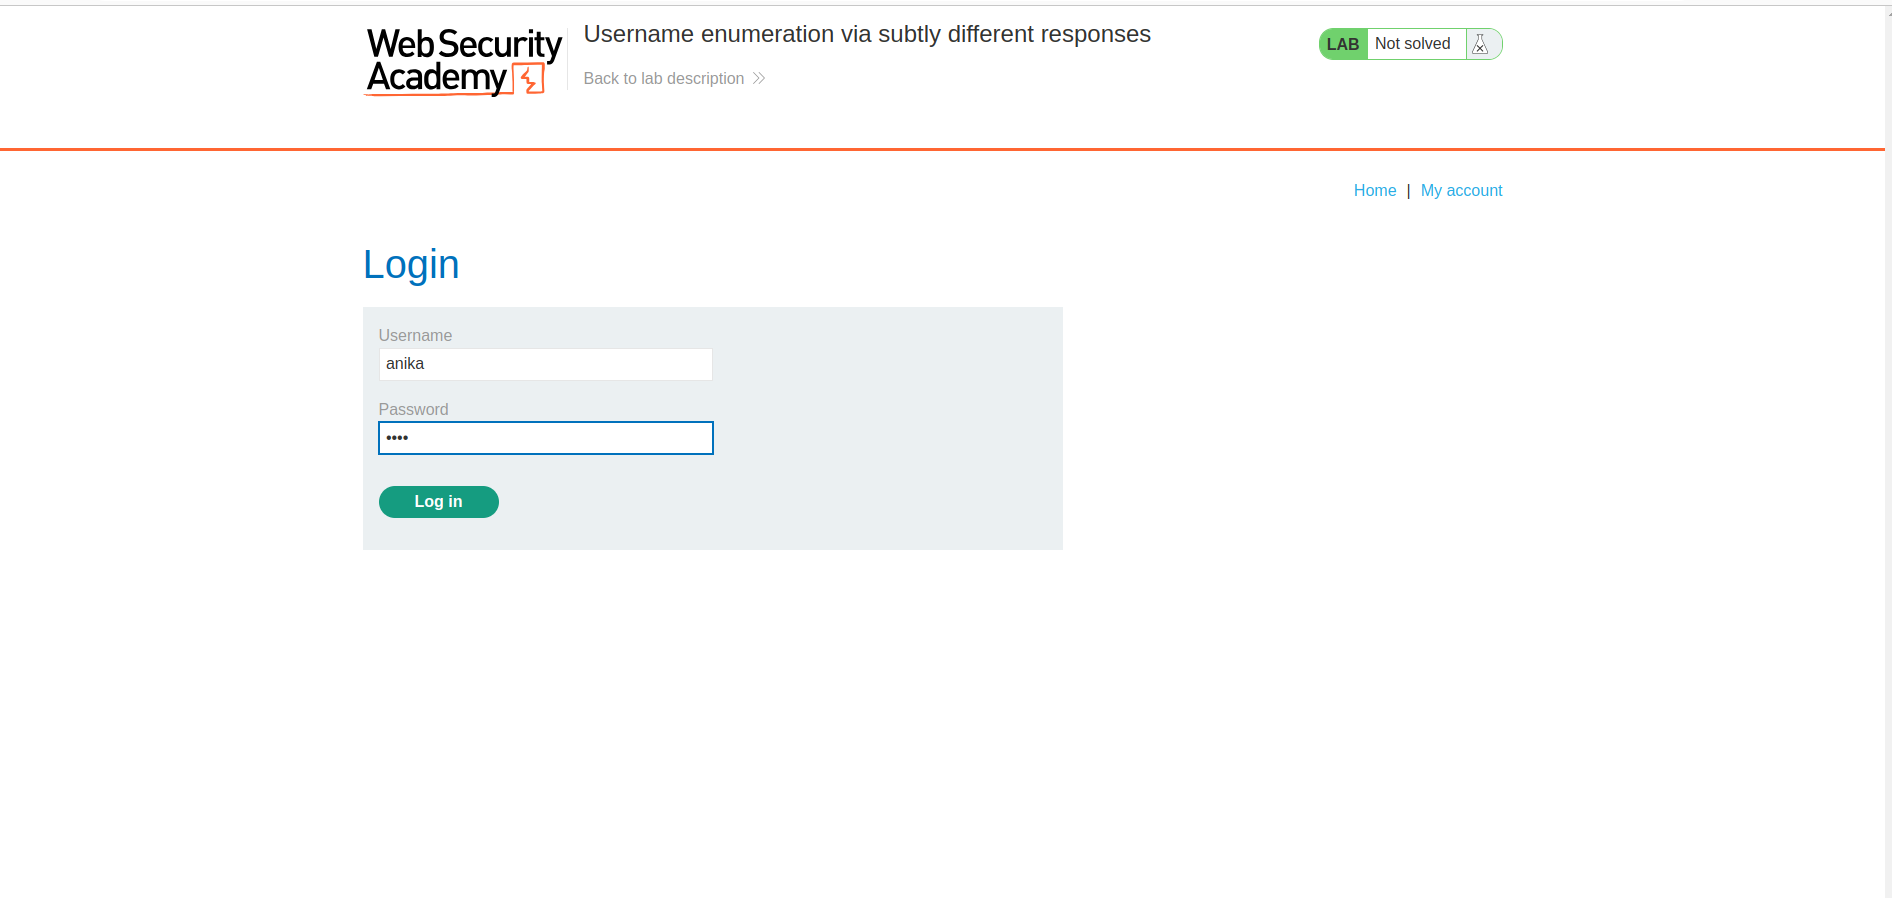
\includegraphics[width=1\textwidth]{Images/anikaScreensots/enumeratinStart.png}
    \caption{trying to login with incorrect usernames and passwords}
    \label{fig:enter-label}
\end{figure}
	

the we will open burp suite and send the request to intruder.   

\begin{figure}[H]
    \centering
    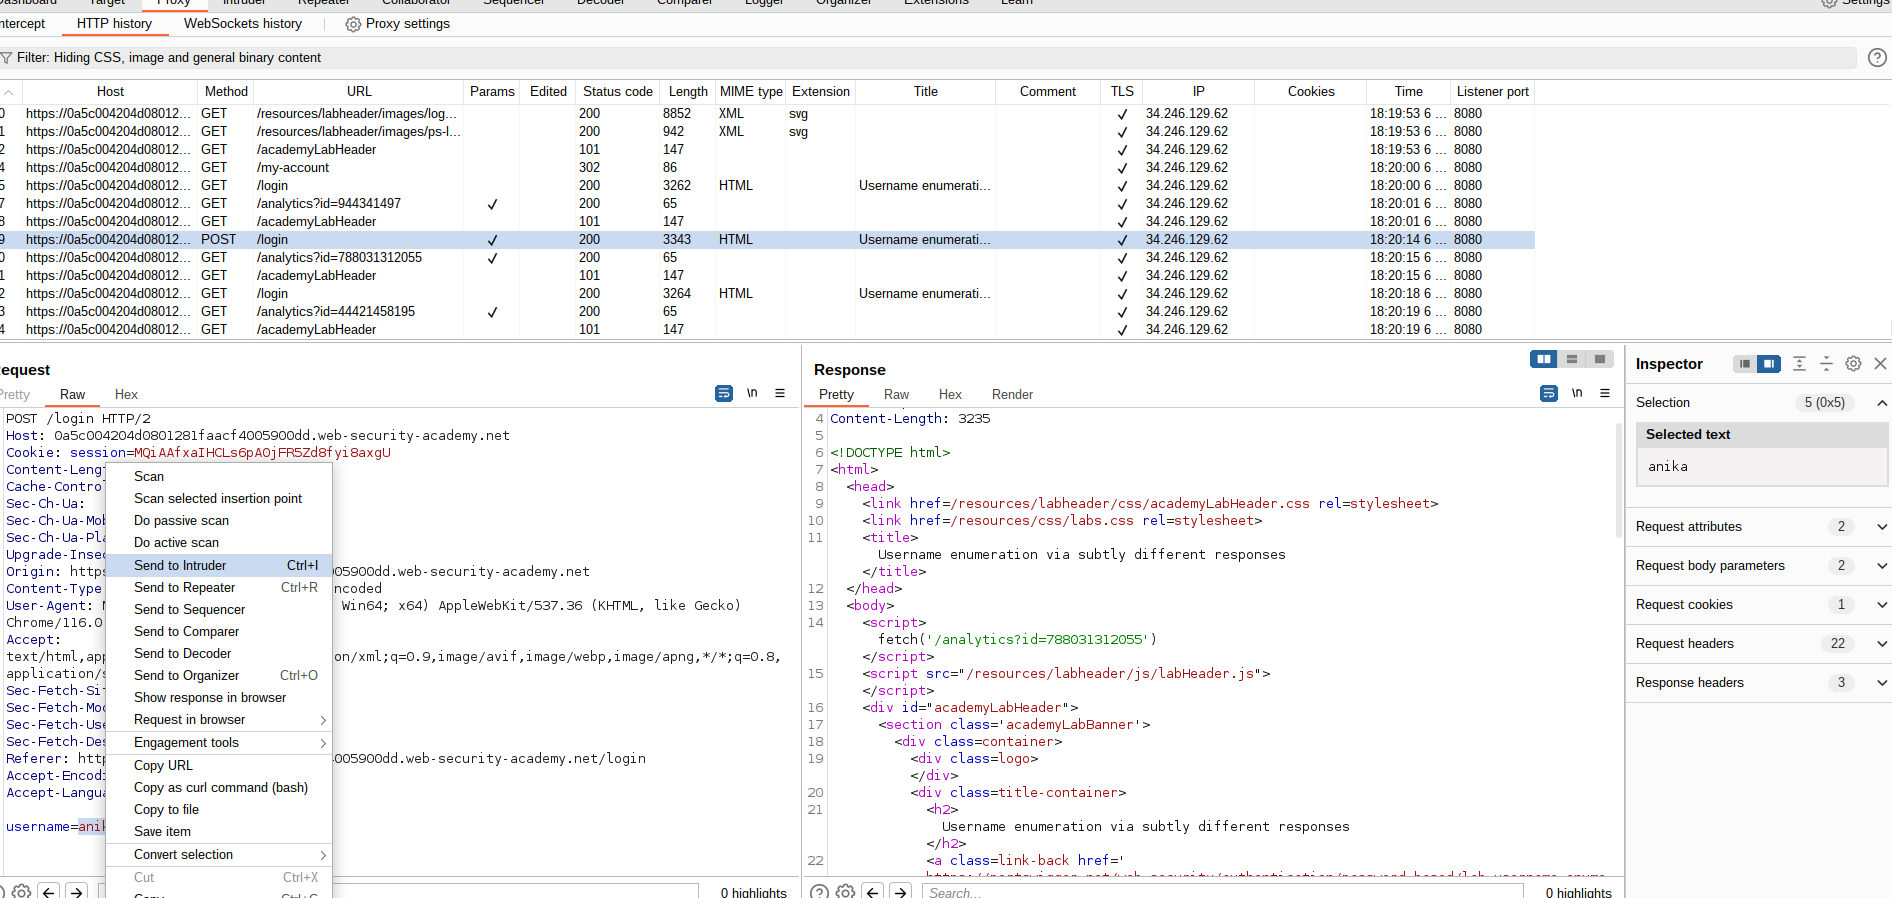
\includegraphics[width=1\textwidth]{Images/anikaScreensots/EnuStep1.png}
    \caption{send the request to intruder}
    \label{fig:enter-label}
\end{figure}

\begin{figure}[H]
    \centering
    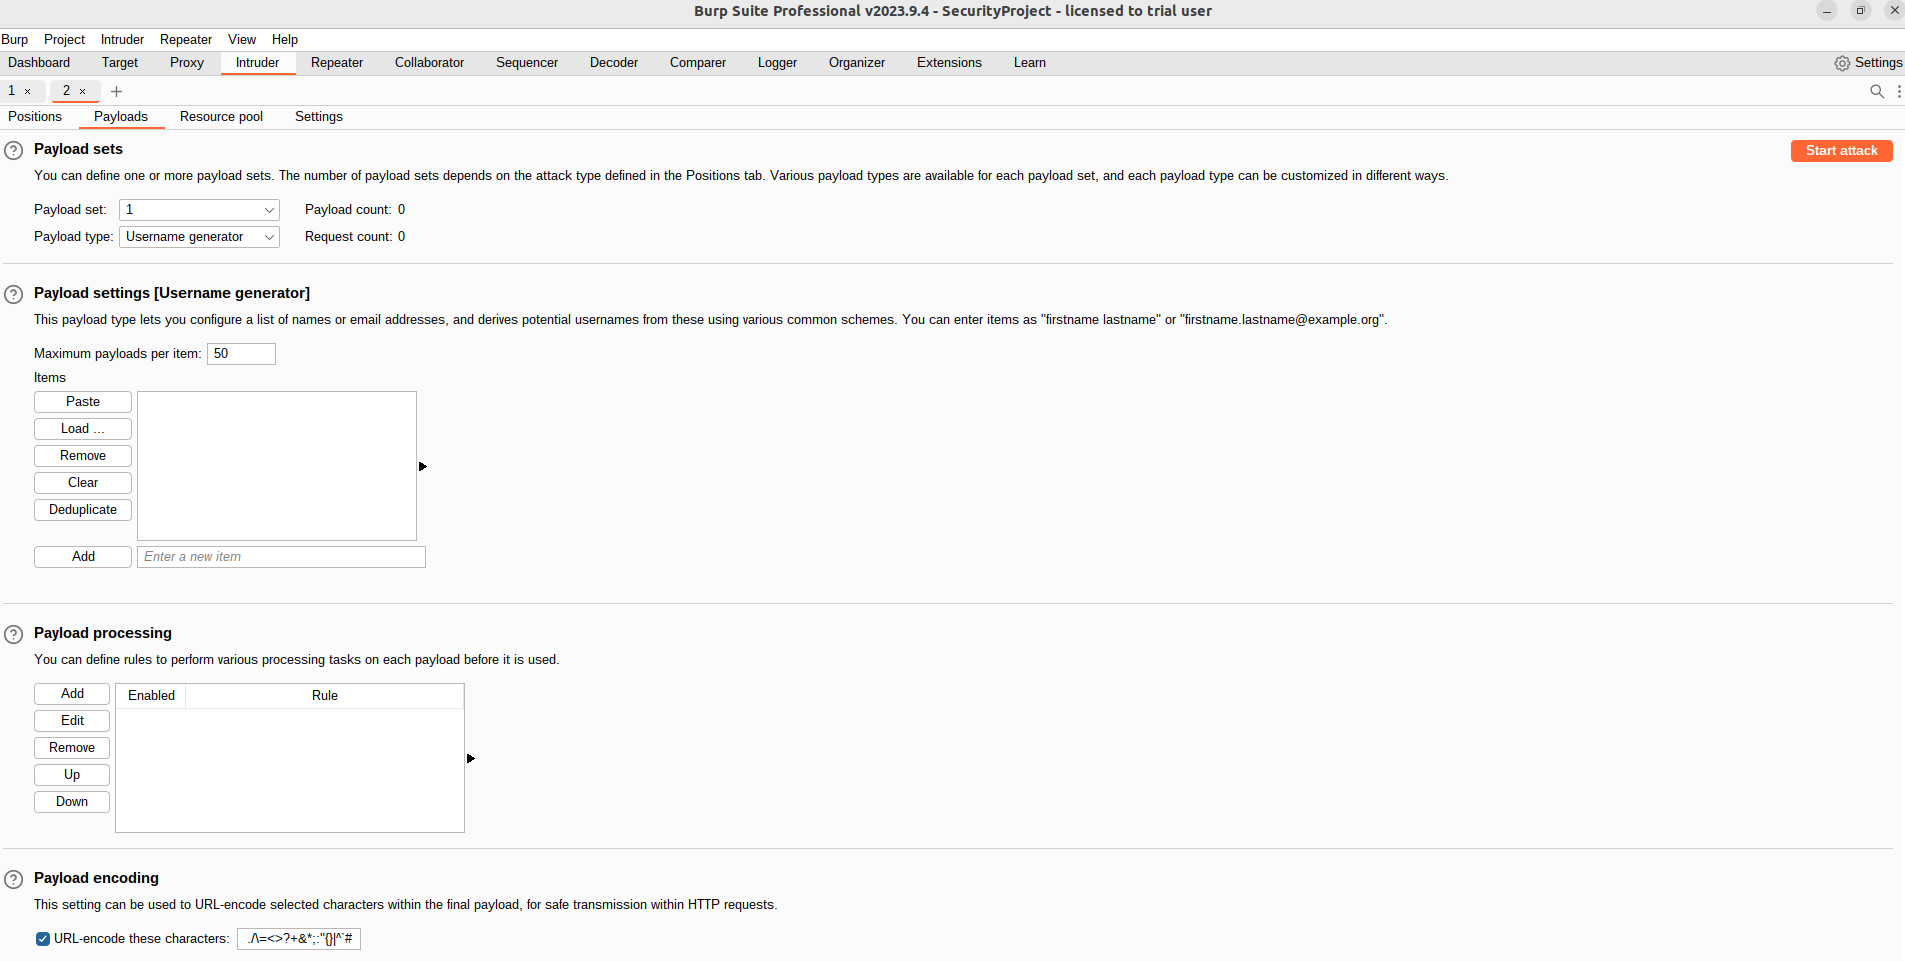
\includegraphics[width=1\textwidth]{Images/anikaScreensots/STEP2.png}
    \caption{setting the payload}
    \label{fig:enter-label}
\end{figure}


 

and click on start attack.

%----------------------------------------------------------------------------------------
%	QUOTATIONS
%----------------------------------------------------------------------------------------

\subsection*{Guessing usernames}

\begin{fullwidth}If we know an user, we can use that name to generate user names based on that knowledge. From the payload type we will use username generator – we can enter the number of usernames we ] want Burp to generate into the maximum payloads per item. For exam, if we know that the name of the attacker is anika monir- burp can generate monir.anika, anikamonir,  anika\textunderscore monir and so on.
\end{fullwidth}

\begin{figure}[H]
    \centering
    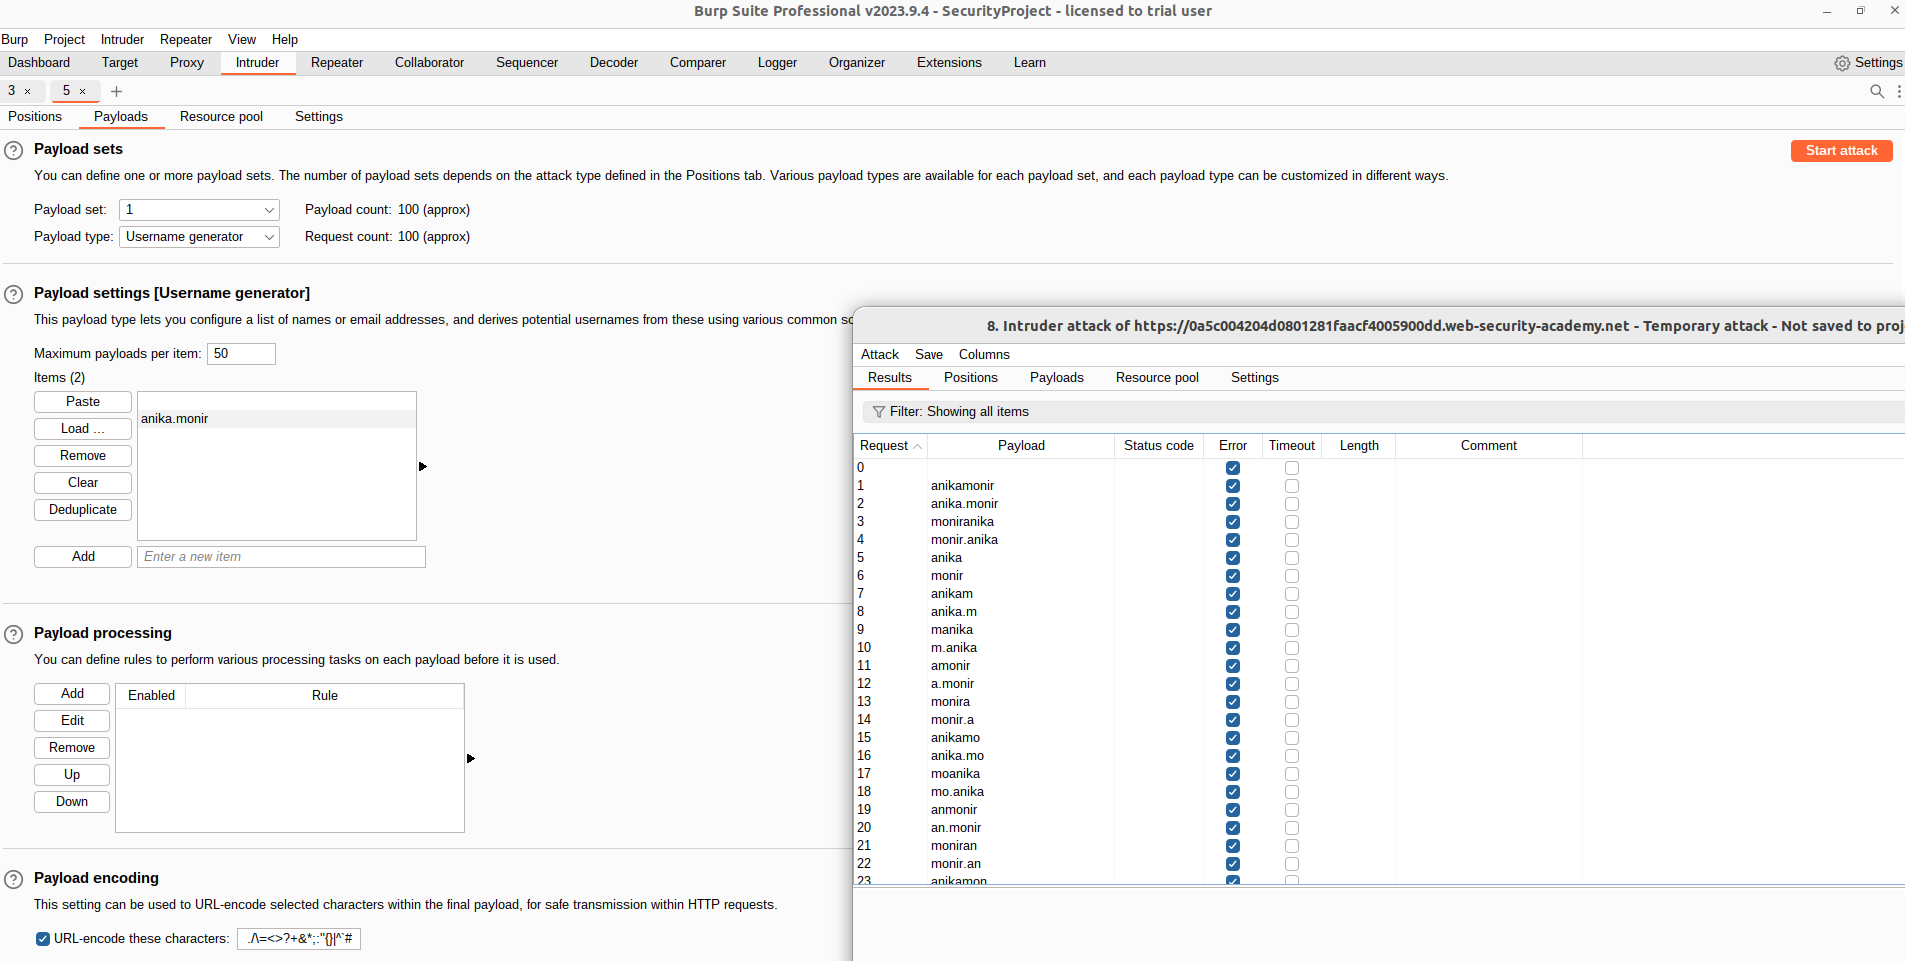
\includegraphics[width=1\textwidth]{Images/anikaScreensots/username.png}
    \caption{implementing the username generator}
    \label{fig:enter-label}
\end{figure}

\subsection*{Brute Forcing Password}
\subsubsection*{Dictionary Attack}
\begin{fullwidth}
    For dictionary attack- We need to make sure that we know at least one valid username. Then we will use a potential list of passwords that we may have gained from previous breach attacks.For example, let’s say we know one username is weiner. Now we will possible passwords from burp suite known password list

\begin{figure}[H]
    \centering
    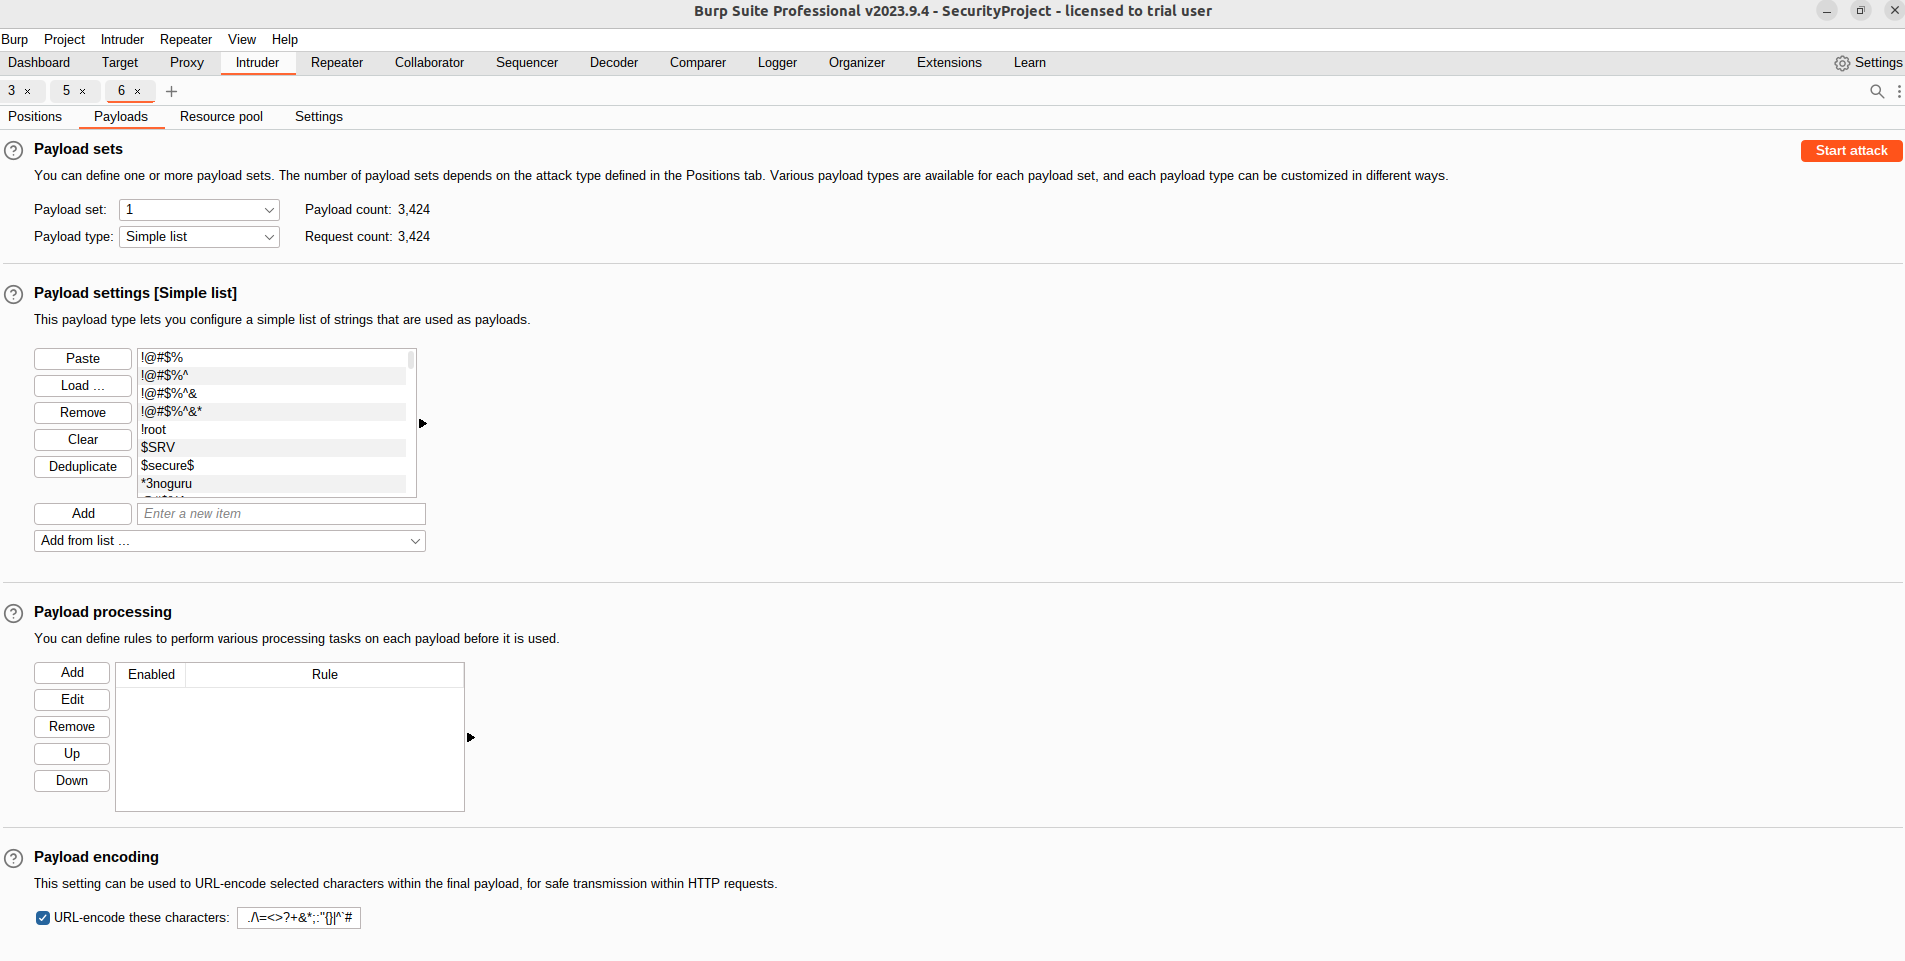
\includegraphics[width=1\textwidth]{Images/anikaScreensots/dictionary1.png}
    \caption{setting the payload a list of known passwords}
    \label{fig:enter-label}
\end{figure}

\begin{figure}[H]
    \centering
    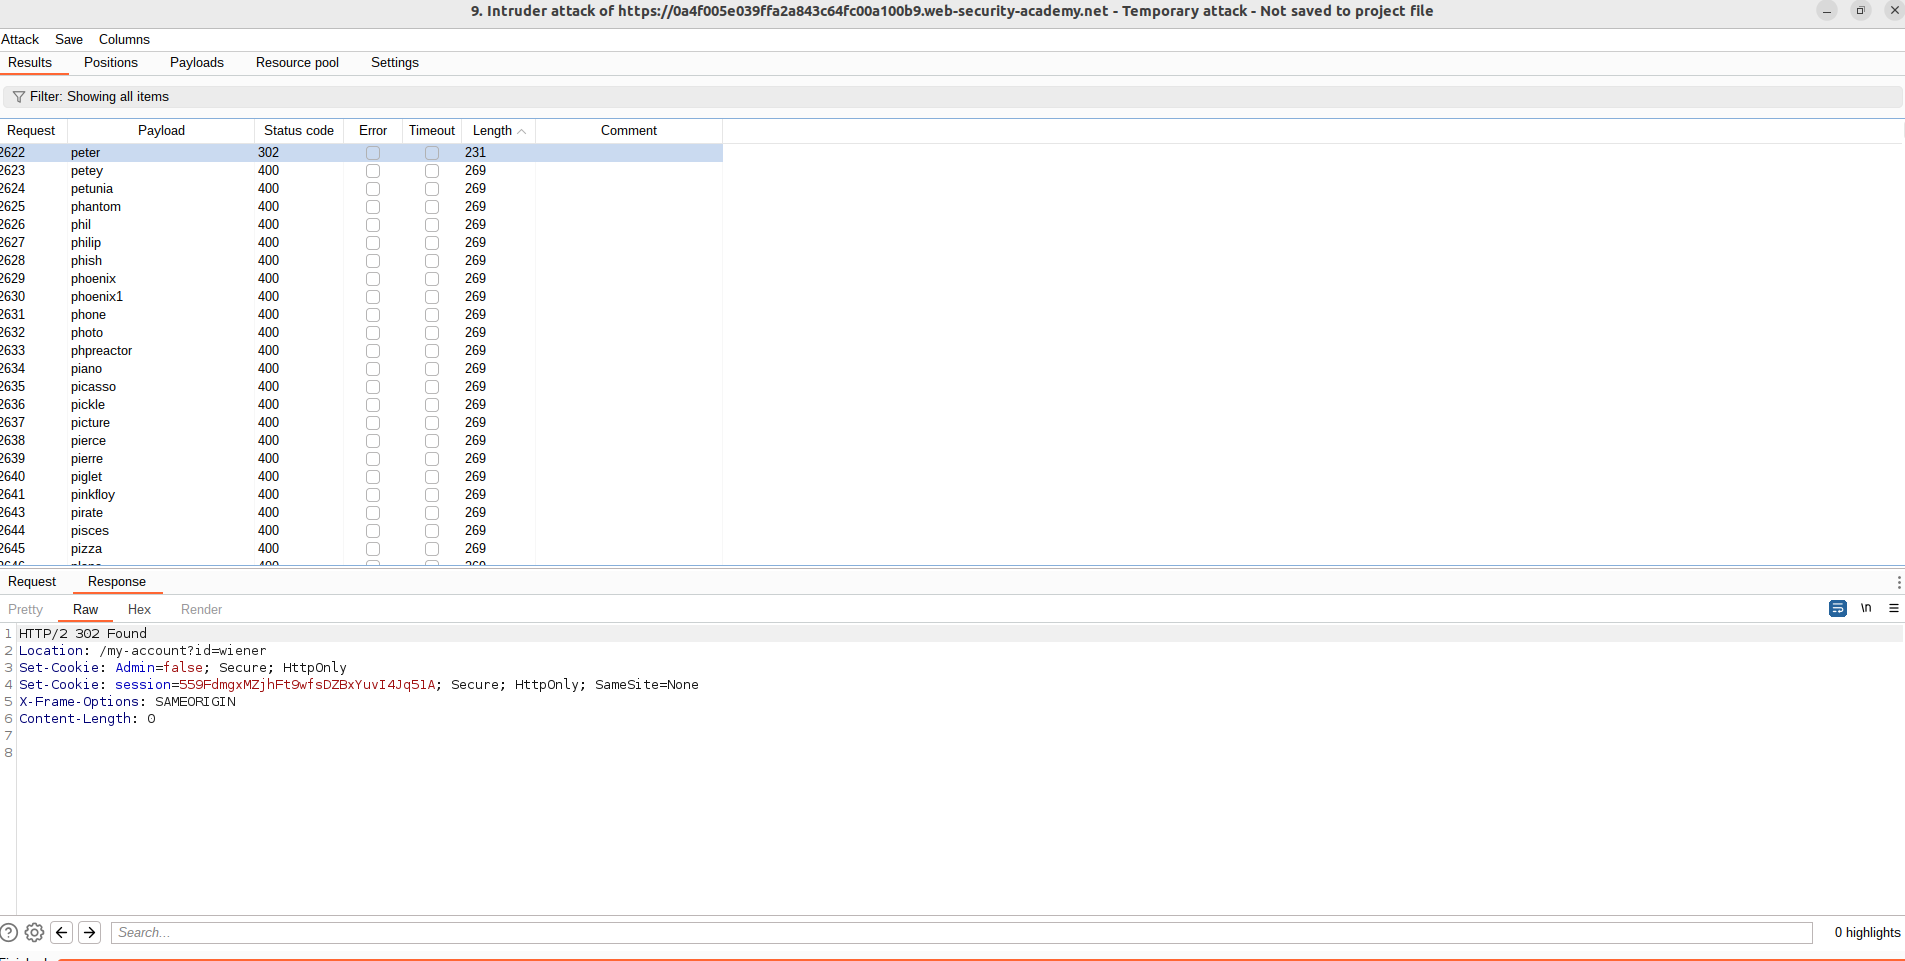
\includegraphics[width=1\textwidth]{Images/anikaScreensots/dictionary2.png}
    \caption{checking the status for different request}
    \label{fig:enter-label}
\end{figure}



\end{fullwidth}
\subsubsection*{Exhaustive Brute Force Attack}
\begin{fullwidth}
    Here we will try every possible combination of character set. This way we will even be able to check for passwords that is uncommon. But we still still need a username that’s valid. Here we can enter the full character set and set the minimum and maximum password length that we want to test for.

    \begin{figure}[H]
    \centering
    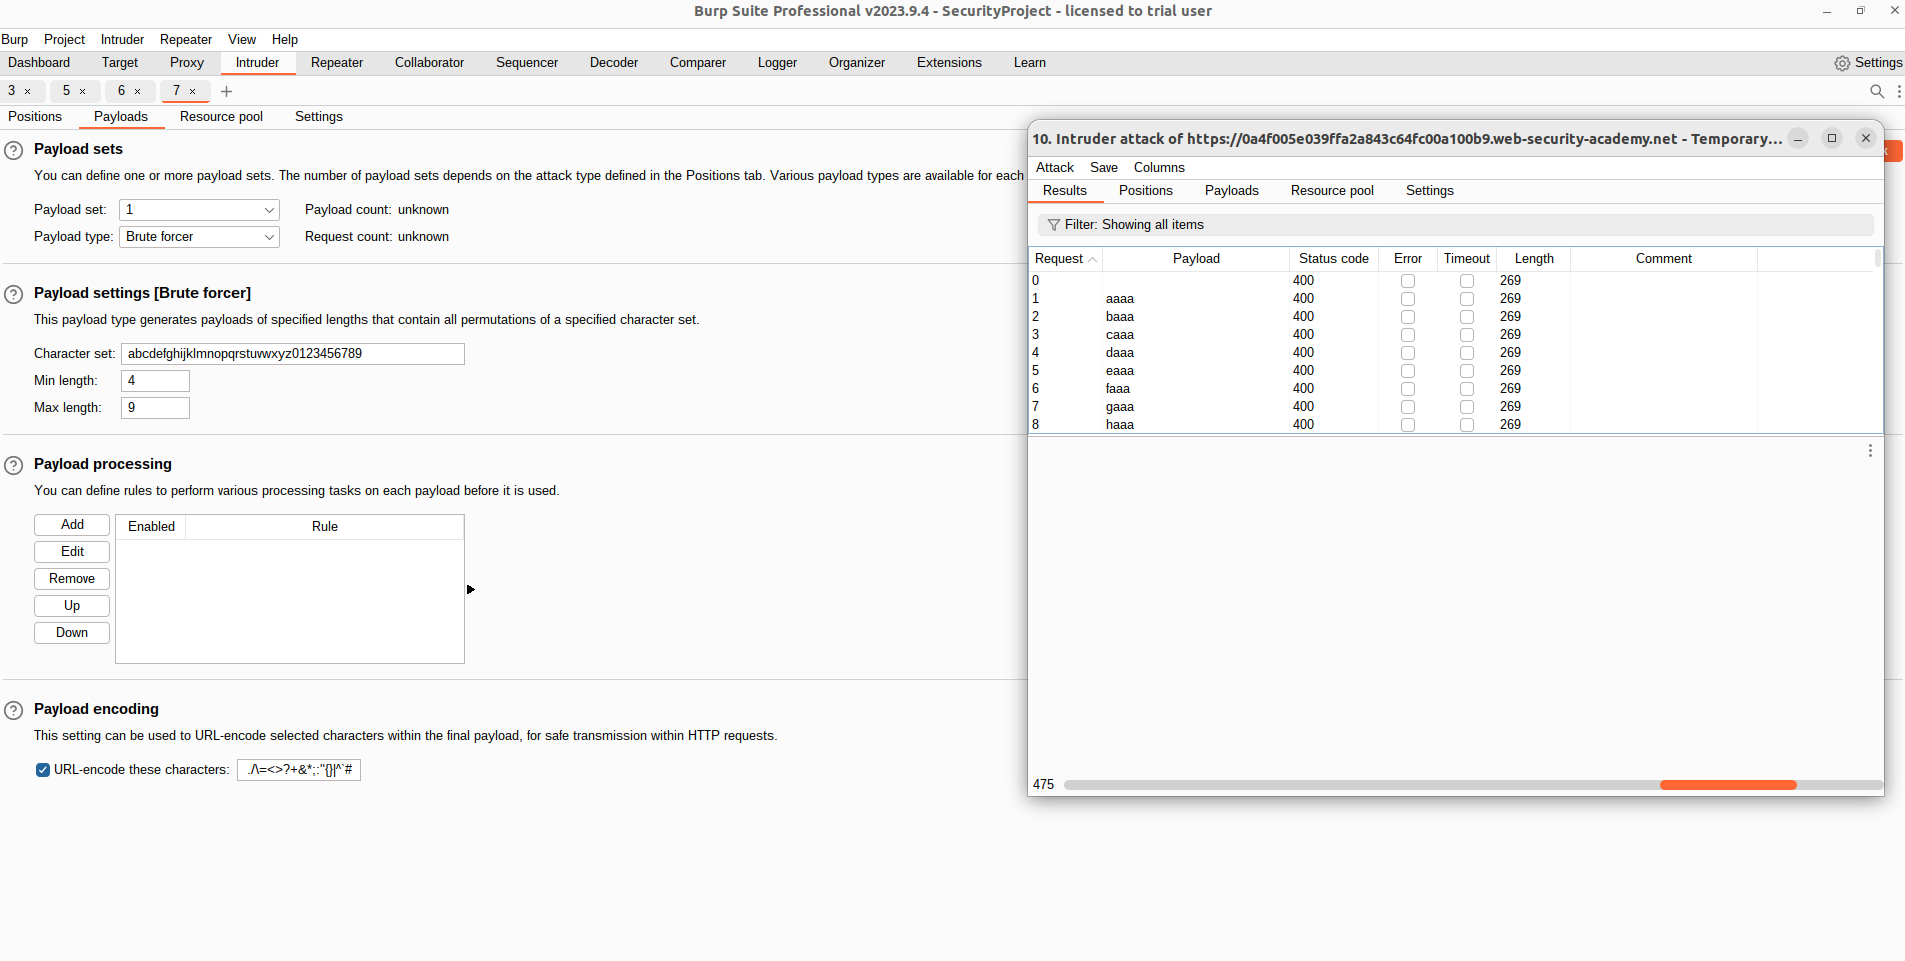
\includegraphics[width=1\textwidth]{Images/anikaScreensots/exaustiveBruteForce.png}
    \caption{}
    \label{fig:enter-label}
\end{figure}
\end{fullwidth}






\subsection*{Credential Stuffing}
\begin{fullwidth}
    Here we use known possible usernames and passwords from websites. This knowledge is usually built up over time from previous breaches. For this we will use the intruder tool and the pitchfork attack type.

    
 \begin{figure}[H]
    \centering
    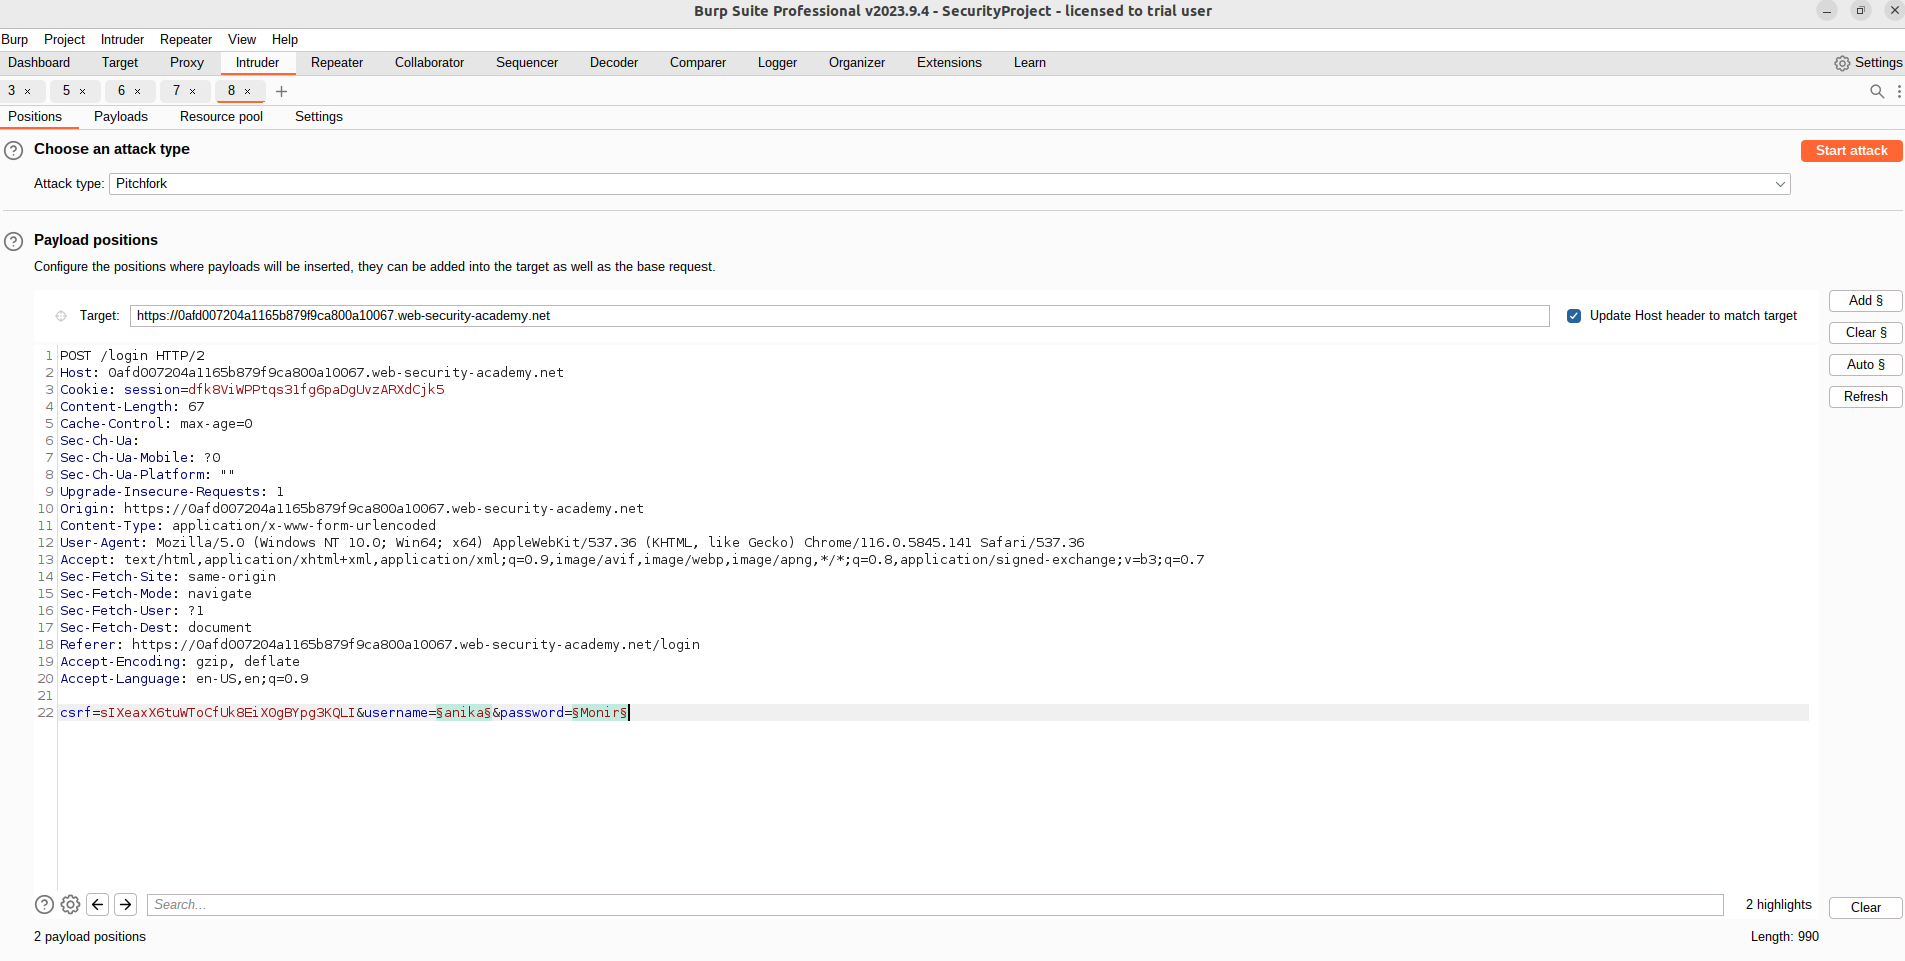
\includegraphics[width=1\textwidth]{Images/anikaScreensots/credentialStuffin1.png}
    \caption{setting the attack type as pitch fork }
    \label{fig:enter-label}
\end{figure}

 \begin{figure}[H]
    \centering
    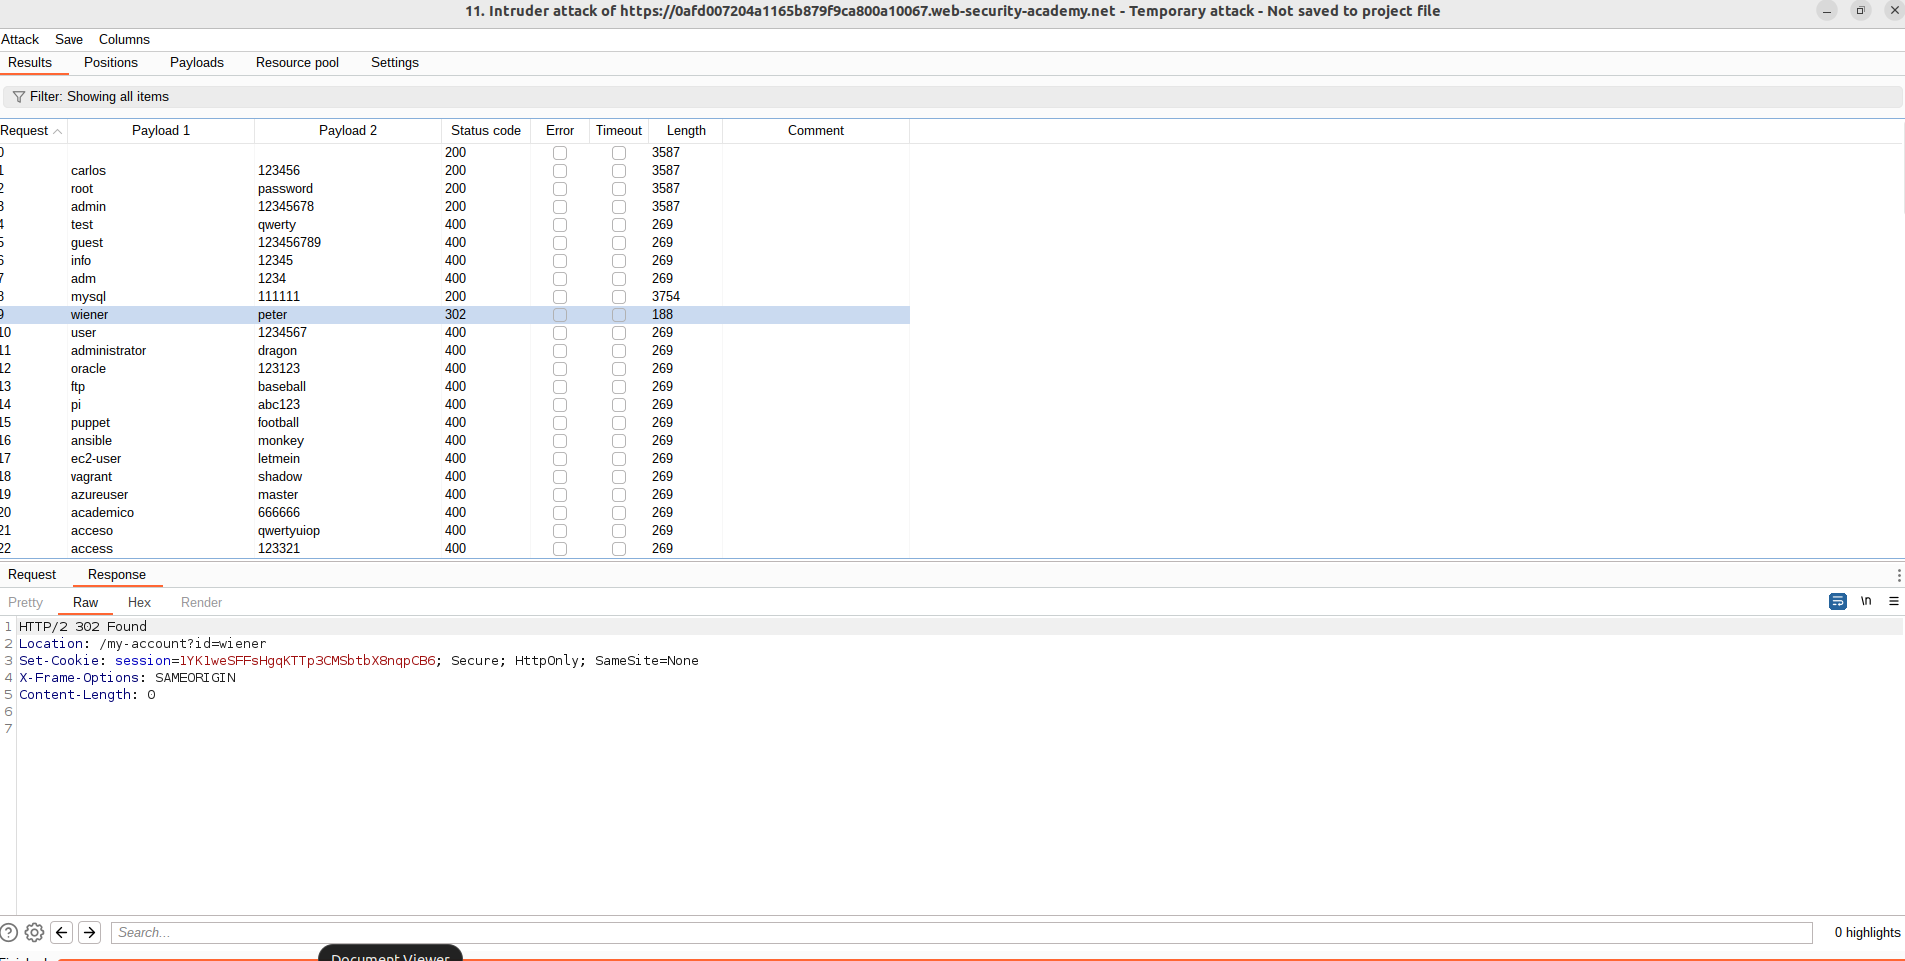
\includegraphics[width=1\textwidth]{Images/anikaScreensots/credentialStuff3.png}
    \caption{setting the payload as known password list from previous breaches}
    \label{fig:enter-label}
\end{figure}

 \begin{figure}[H]
    \centering
    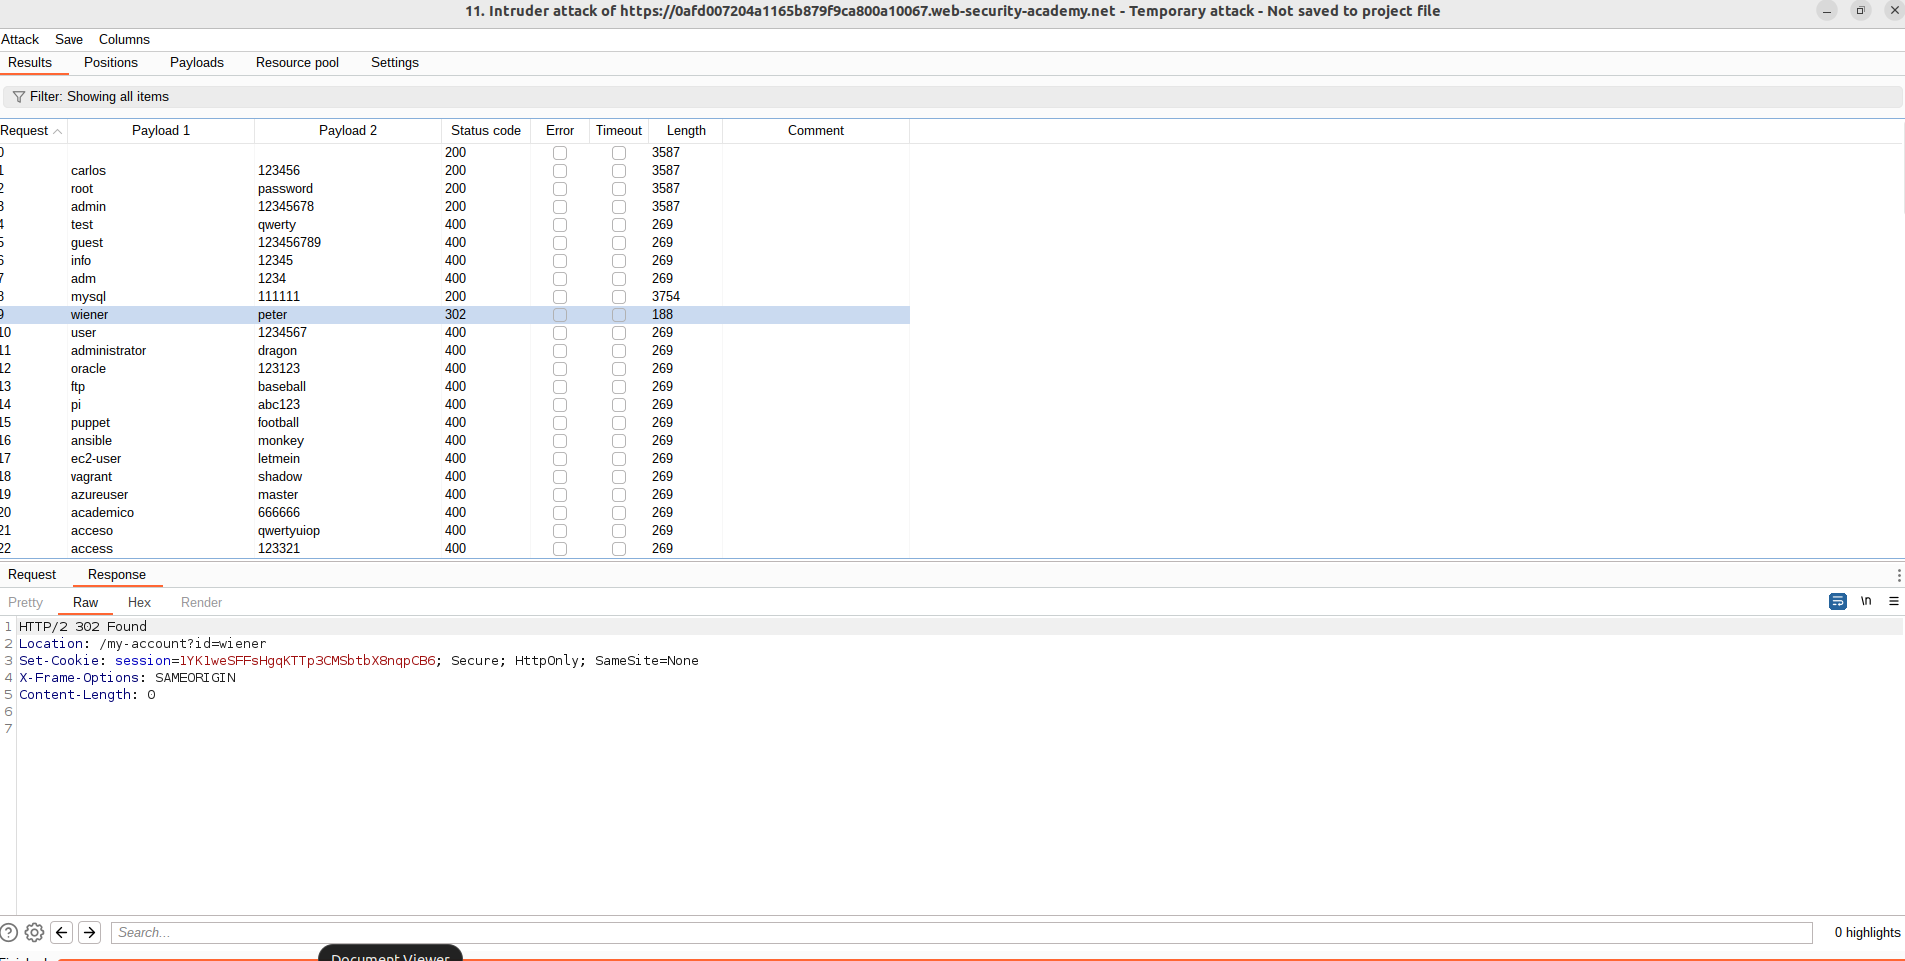
\includegraphics[width=1\textwidth]{Images/anikaScreensots/credentialStuff3.png}
    \caption{checking the response for each request and check for anomalies to gain knowledge}
    \label{fig:enter-label}
\end{figure}
 

\end{fullwidth}
\subsection*{Brute force login}

\begin{fullwidth}
    Since we may not always have any information on usernames and passwords- we can also brute force attacks using the cluster bomb attack type of intruder tool.


     \begin{figure}[H]
    \centering
    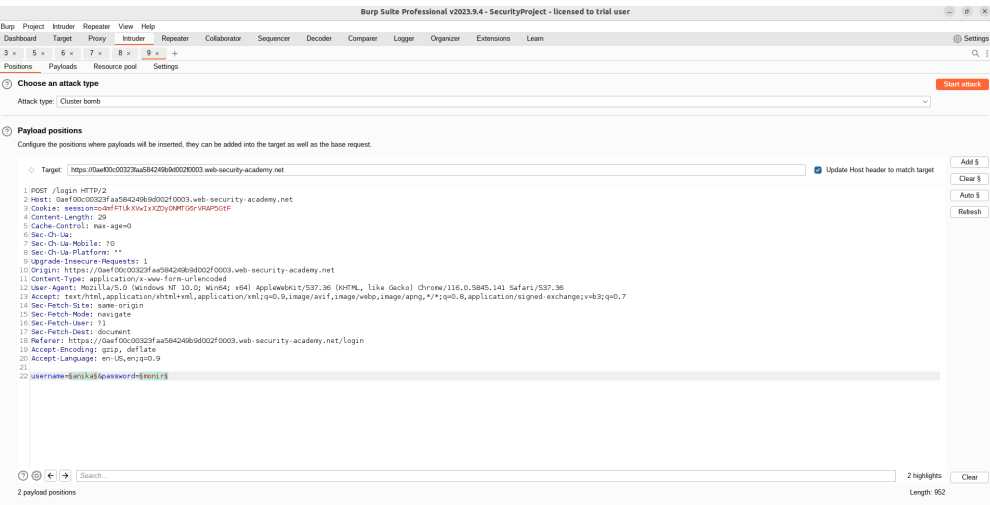
\includegraphics[width=1\textwidth]{Images/anikaScreensots/BruteForce1.png}
    \caption{setting the attack type as pitch fork}
    \label{fig:enter-label}
\end{figure}

 \begin{figure}[H]
    \centering
    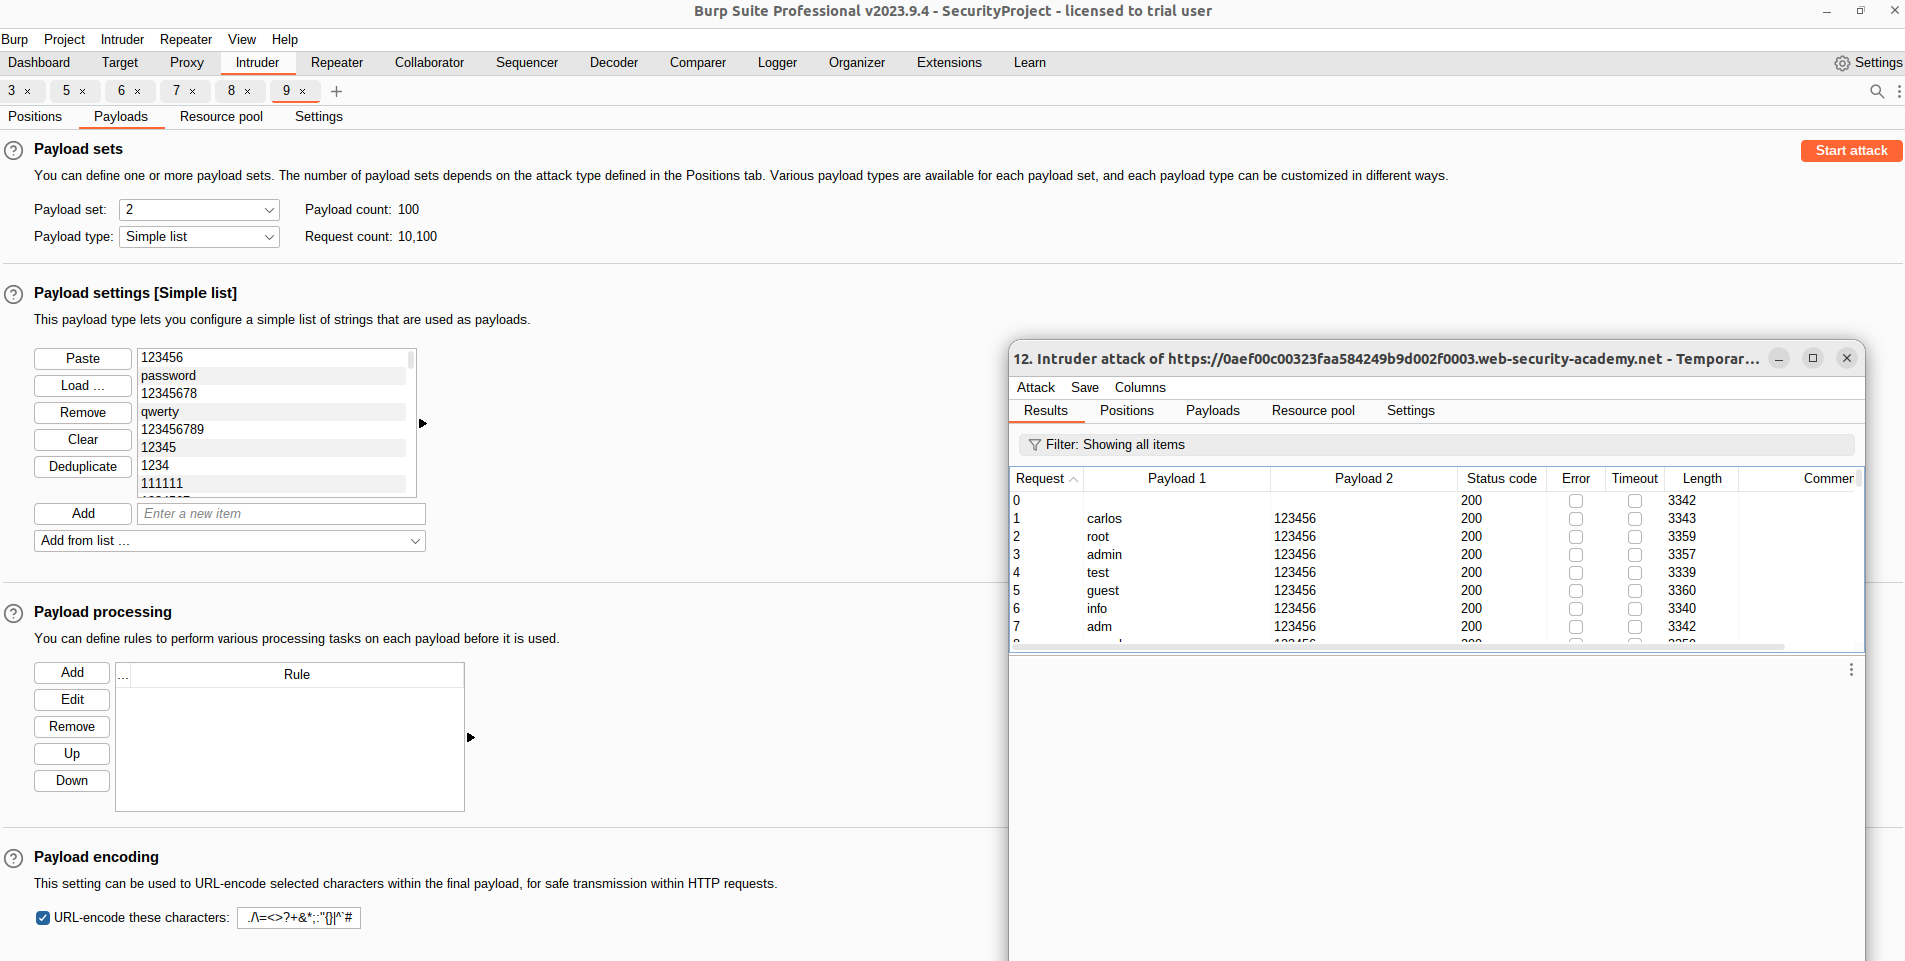
\includegraphics[width=1\textwidth]{Images/anikaScreensots/bruteForce2.png}
    \caption{setting the payload as known password list from previous breaches}
    \label{fig:enter-label}
\end{figure}

 \begin{figure}[H]
    \centering
    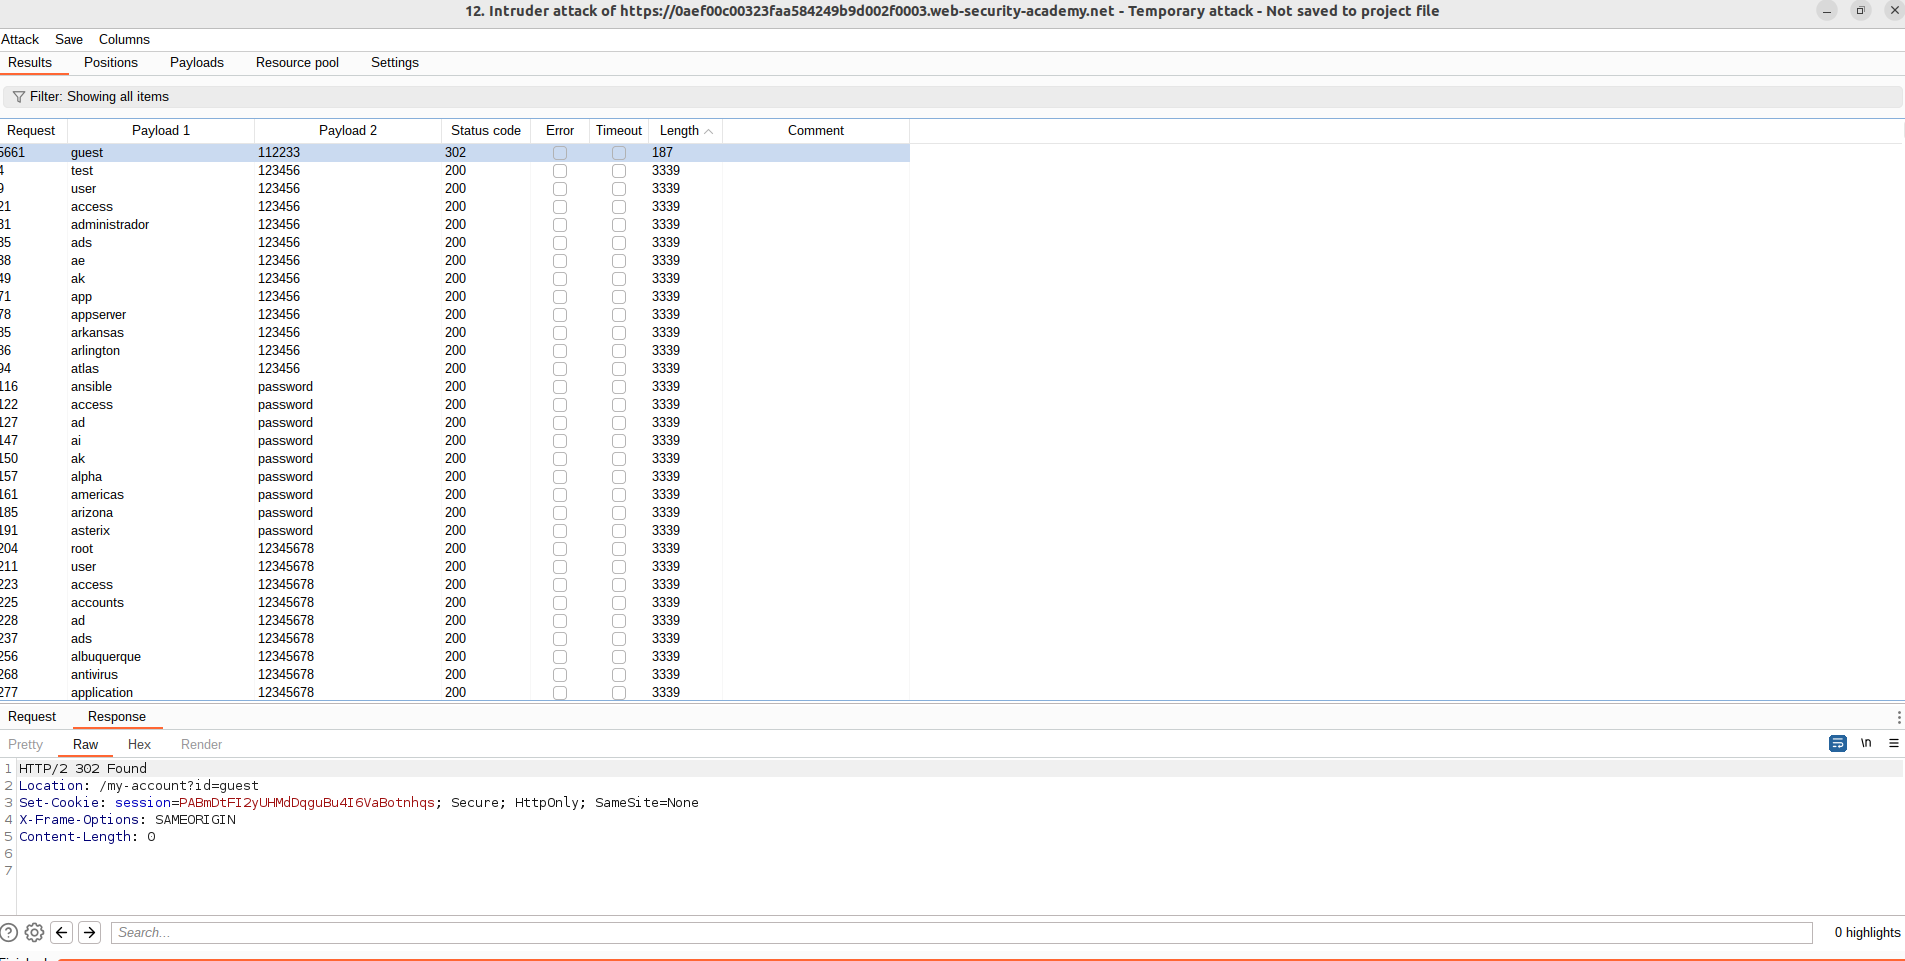
\includegraphics[width=1\textwidth]{Images/anikaScreensots/bruteForce3.png}
    \caption{checking the response for each request and check for anomalies to gain knowledge}
    \label{fig:enter-label}
\end{figure}

\end{fullwidth}
\subsection*{Privilege escalation}
\begin{fullwidth}
    
When a user logs in to an application, they usually only have access to the parts of the application that they need to perform their specific tasks. If access controls are incorrectly set, a user can gain access to functionality that should only be available to higher-privileged users.


\begin{figure}[H]
    \centering
    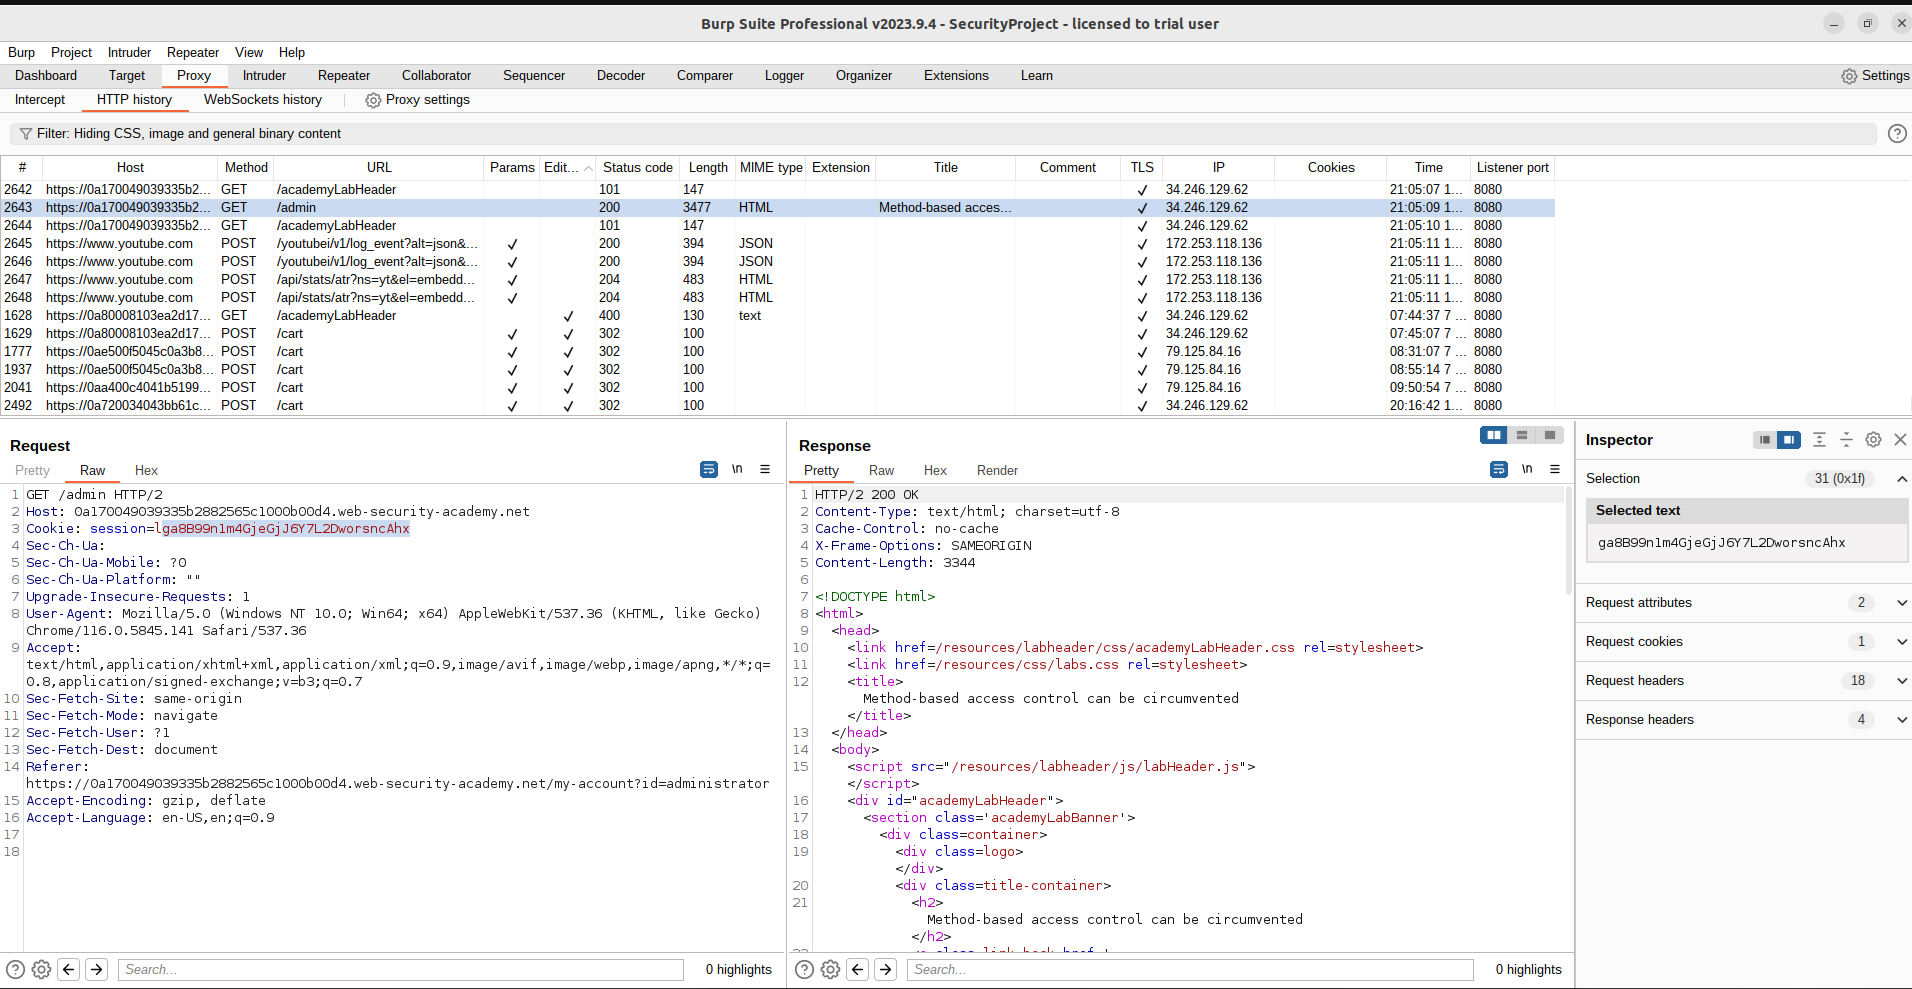
\includegraphics[width=1\textwidth]{Images/anikaScreensots/prev1.png}
    \caption{log in as an administrator and access the admin panel}
    \label{fig:enter-label}
\end{figure}


\begin{figure}[H]
    \centering
    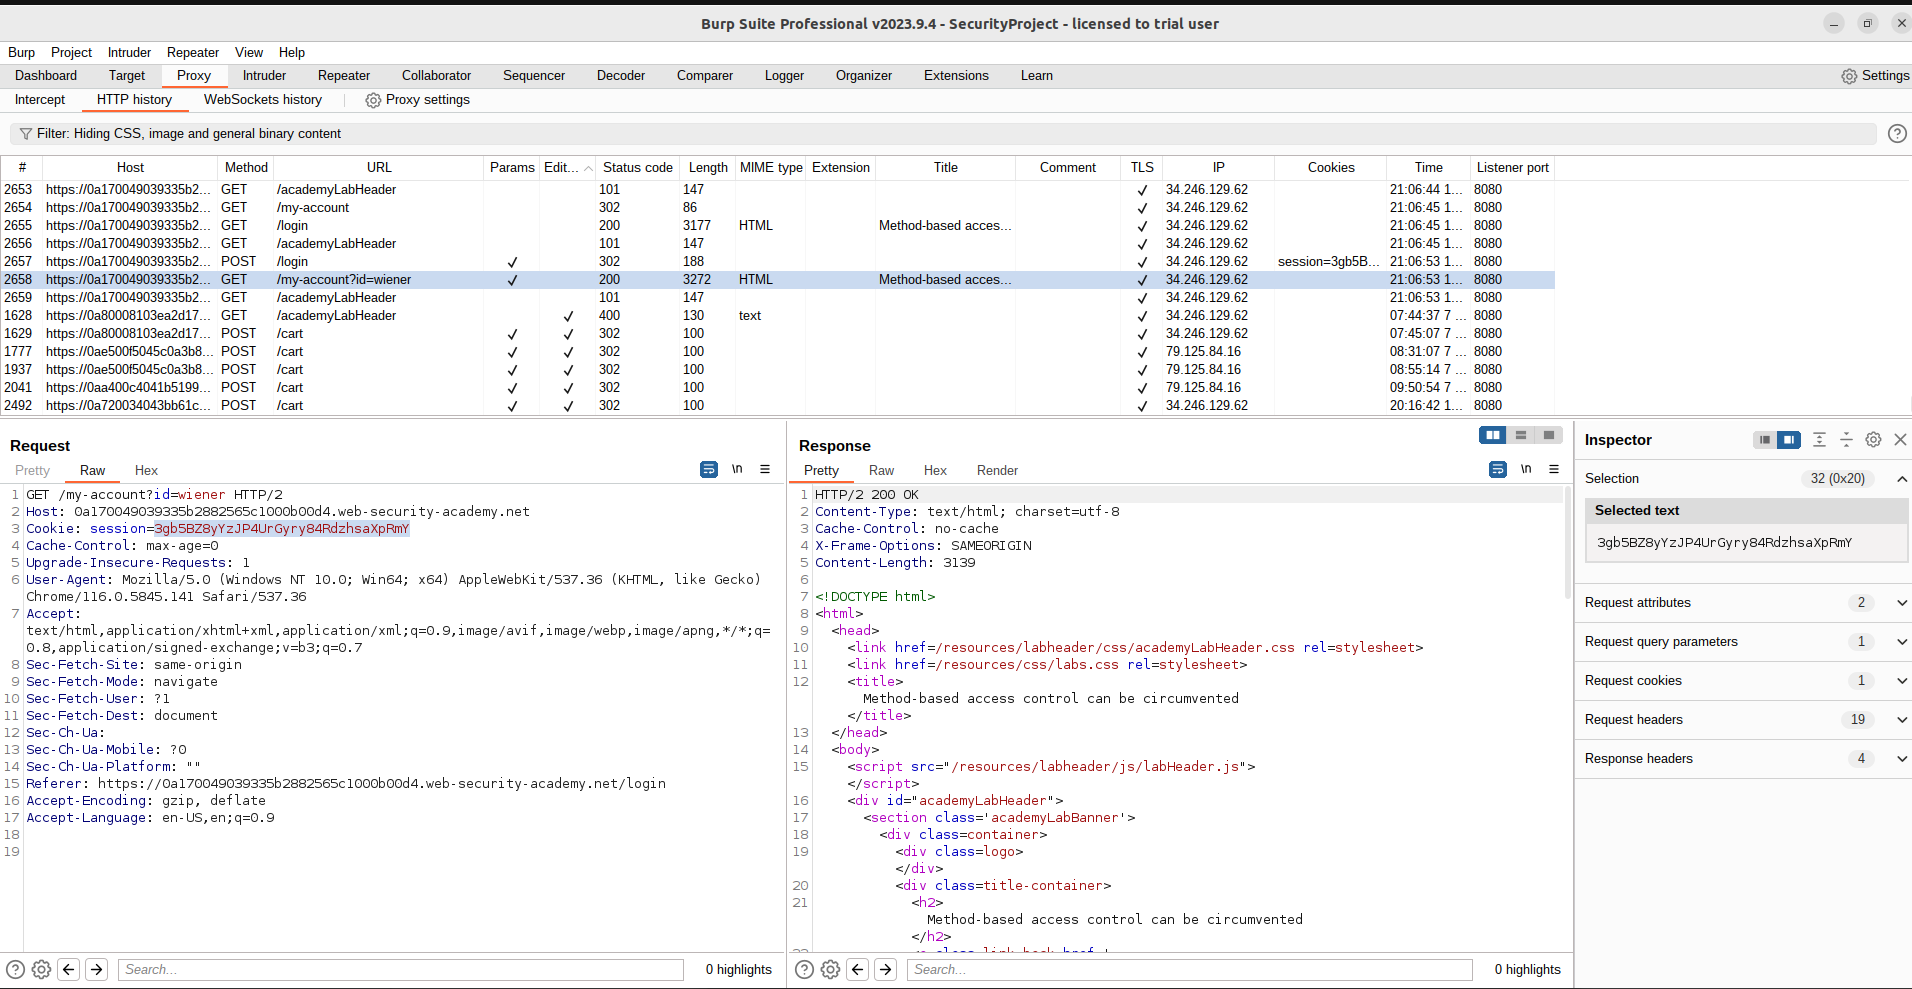
\includegraphics[width=1\textwidth]{Images/anikaScreensots/prev2.png}
    
    \caption{login as a normal user}
    \label{fig:enter-label}
\end{figure}

\begin{figure}[H]
    \centering
    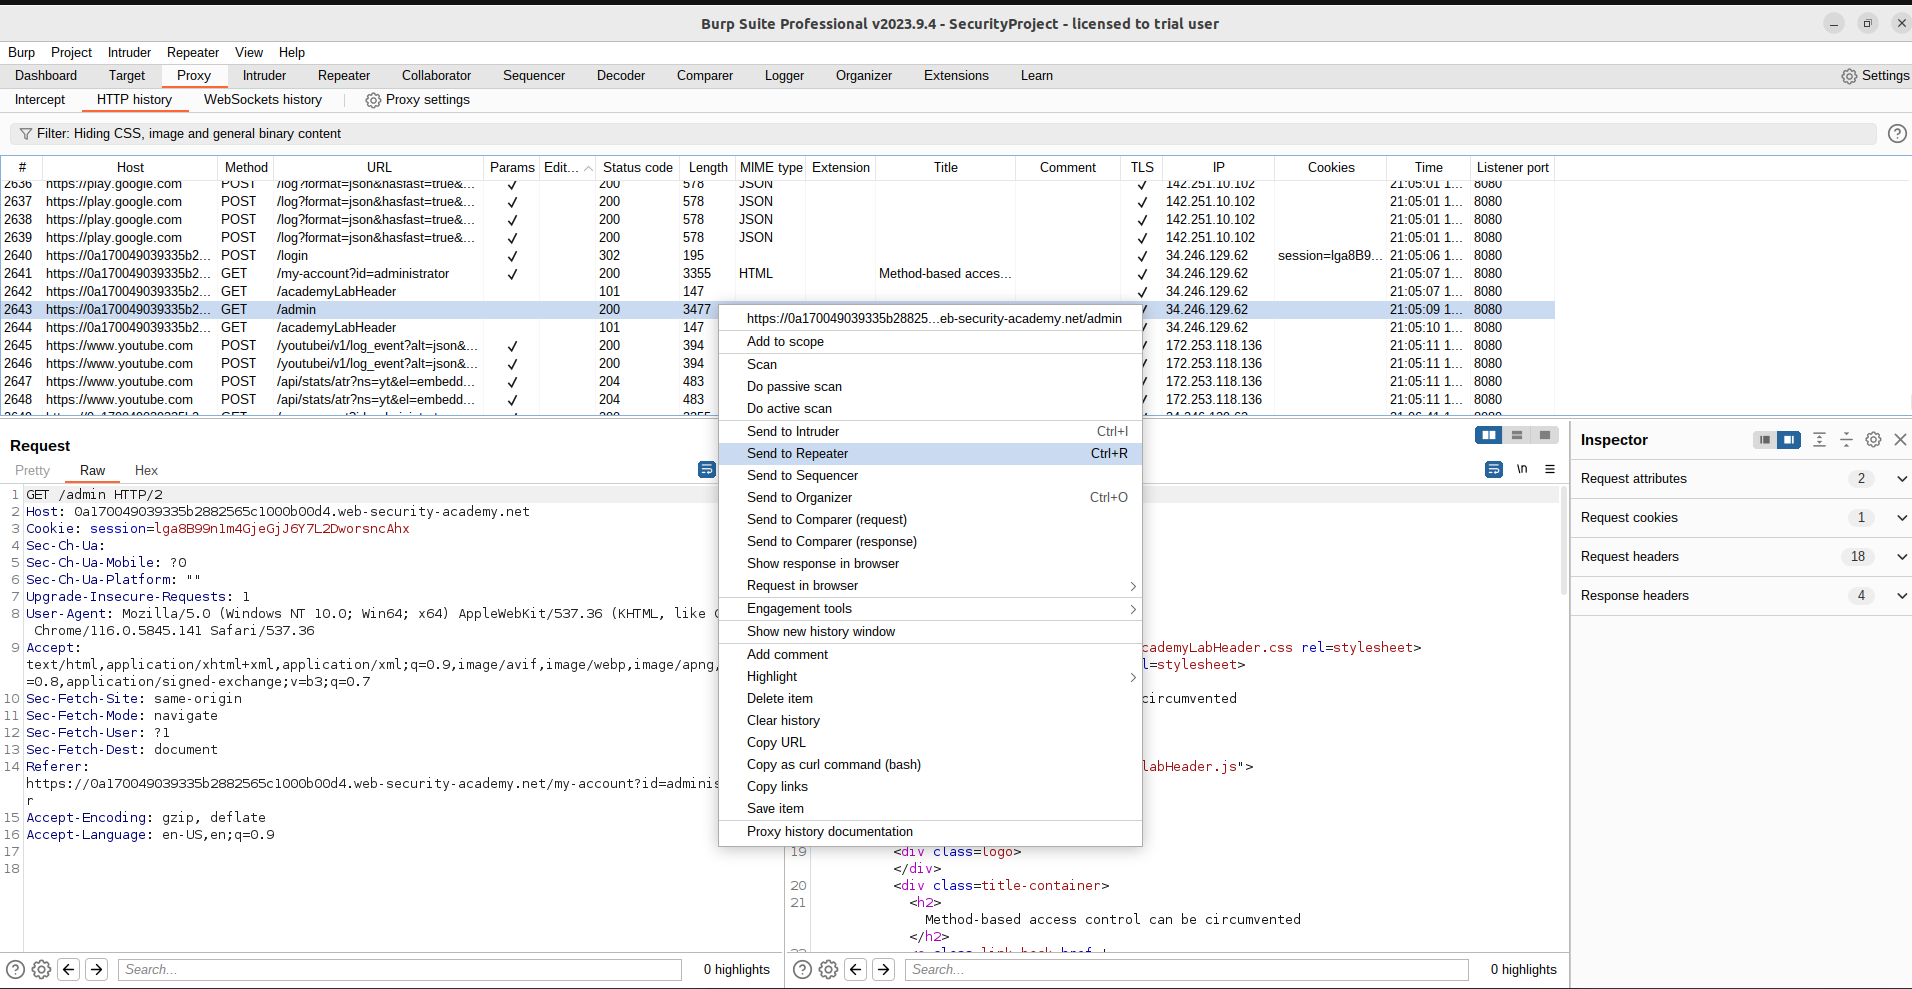
\includegraphics[width=1\textwidth]{Images/anikaScreensots/prev3.png}
    \caption{send the recent request of normal user to repeater}
    \label{fig:enter-label}
\end{figure}

\begin{figure}[H]
    \centering
    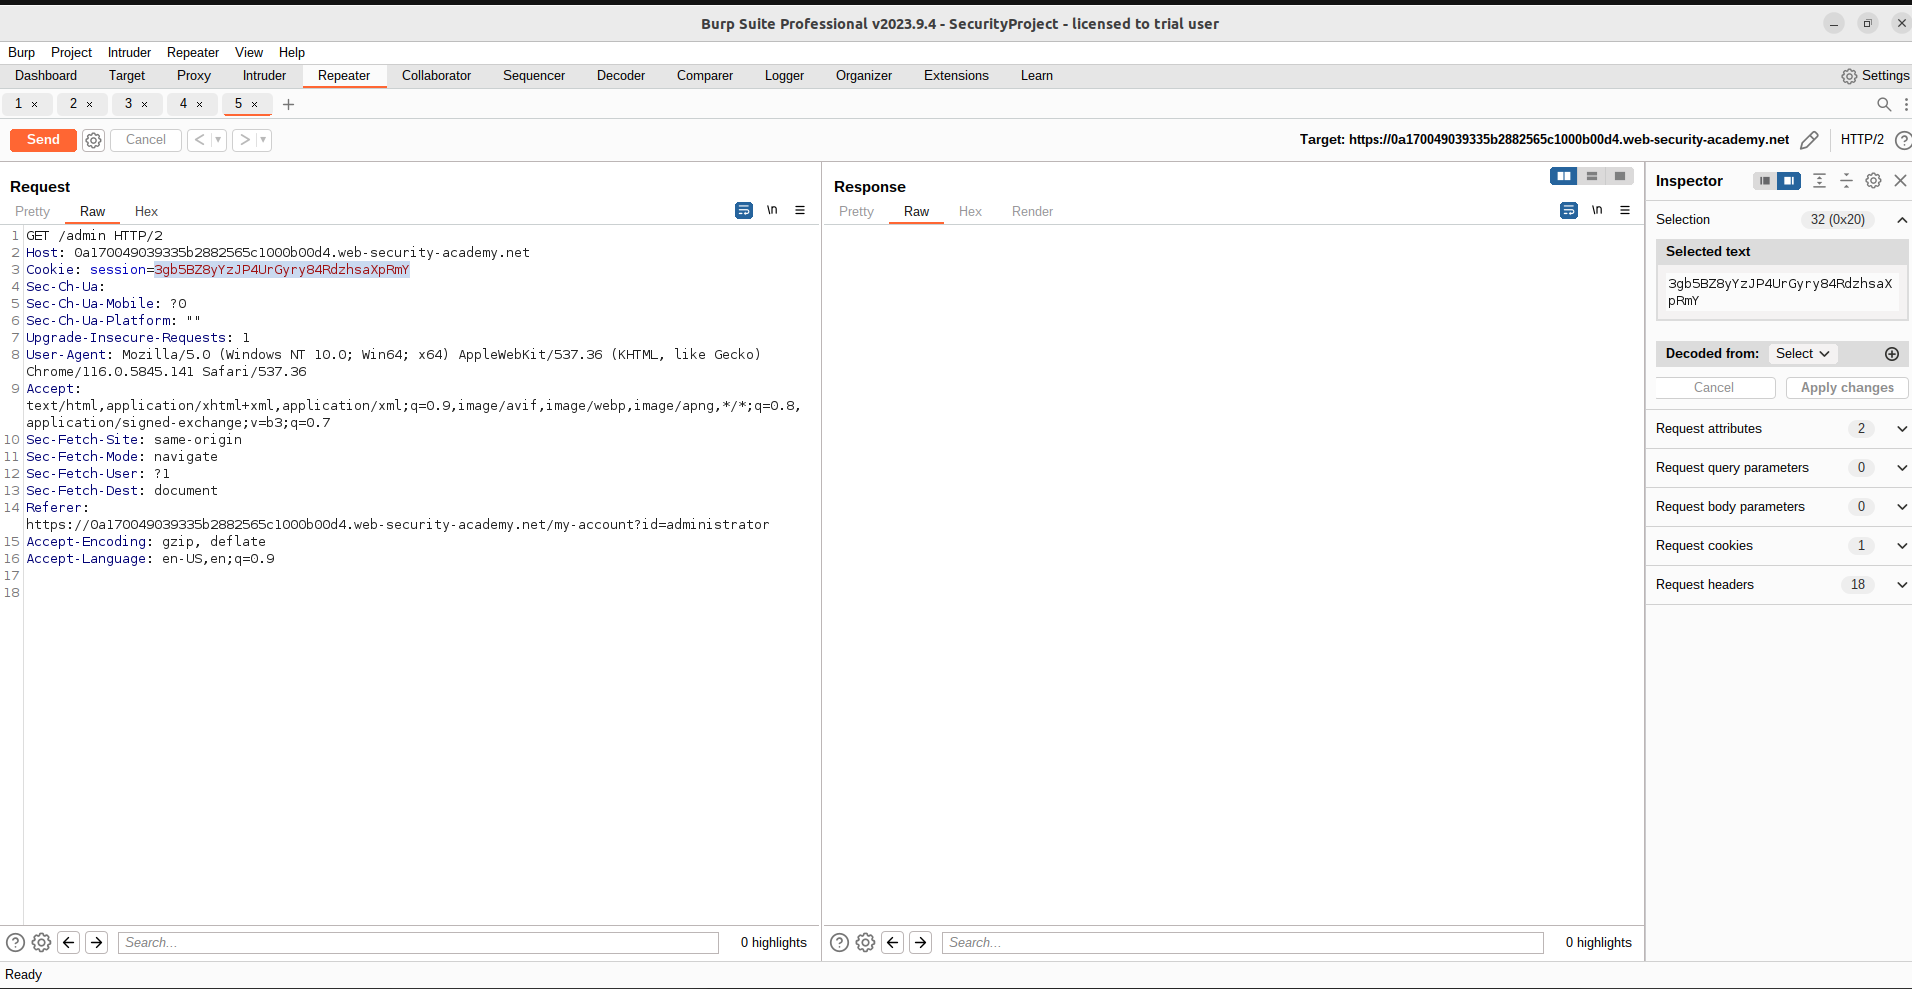
\includegraphics[width=1\textwidth]{Images/anikaScreensots/prev4.png}
    \caption{copy the session cookie of normal user to the administrative user}
    \label{fig:enter-label}
\end{figure}


\begin{figure}[H]
    \centering
    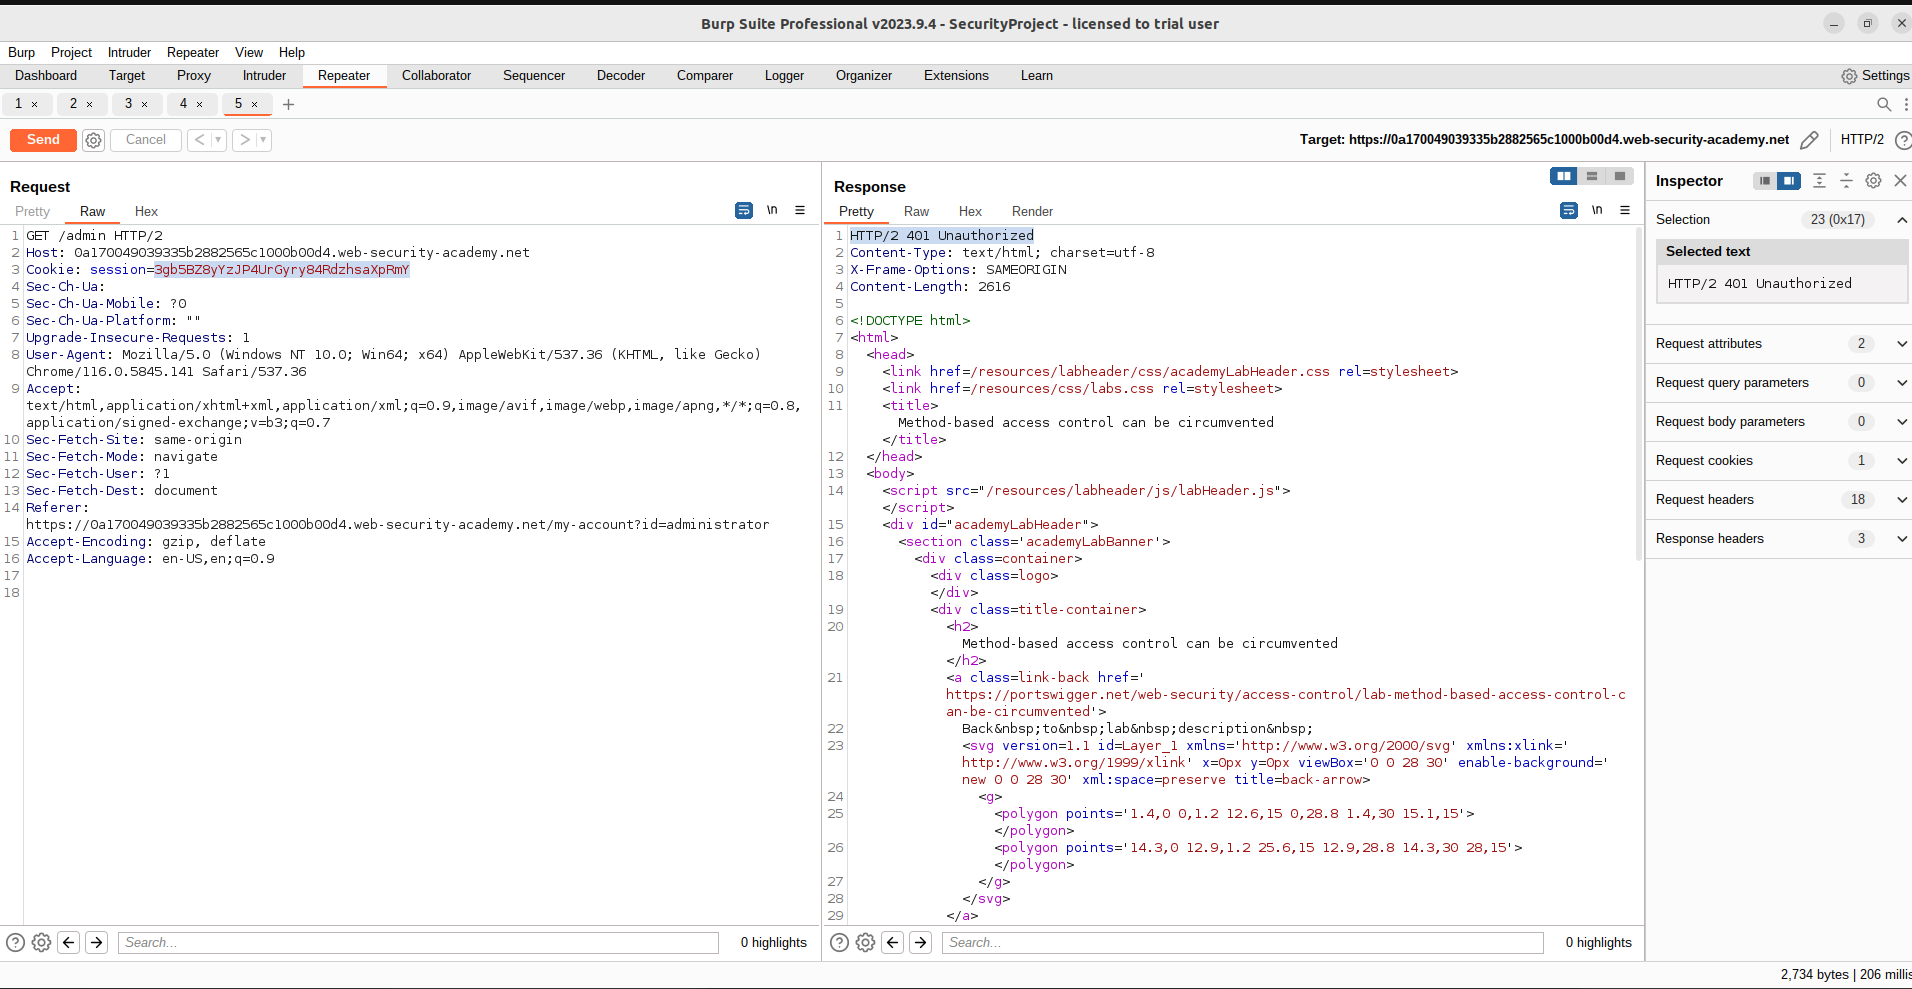
\includegraphics[width=1\textwidth]{Images/anikaScreensots/prev5.png}
    \caption{send the request and check if the security breach works.Here we got a 401 confirming that the endpoint is not vulnerable}
    \label{fig:enter-label}
\end{figure}

\end{fullwidth}
%----------------------------------------------------------------------------------------
%	Penetration testing workflow - Testing for vulnerabilities - Testing SQL Injection vulnerabilities
%----------------------------------------------------------------------------------------
\addcontentsline{toc}{subsubsection}{Testing SQL Injection vulnerabilities}
\subsubsection*{Testing SQL Injection vulnerabilities}
SQL injection is a web security vulnerability that allows an attacker to interfere with the queries that an application makes to its database. It generally enables an attacker to view data that they are not normally able to retrieve. An attacker may then be able to modify or delete this data. \newline

For this, let test for this educational lab : \href{https://portswigger.net/web-security/sql-injection/lab-retrieve-hidden-data}{\color{orange}sql\textunderscore injection\textunderscore lab}

\begin{itemize}
    \item select category All 
    \item Then go to the browser and select any category.
    \begin{figure}[H]
        \centering
        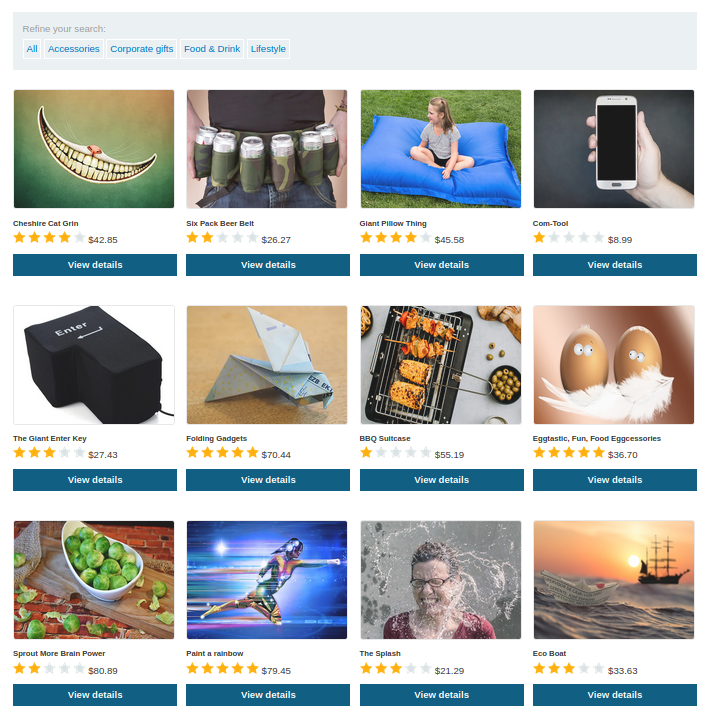
\includegraphics[width=1\linewidth]{Images//sql injection/category_all.png}        
    \end{figure}
    \item So, this is all the website shows us.
    \item now turn on the intercept in proxy 
    \item select any category. and go to {\color{orange}\textbf{Proxy}} > {\color{orange}\textbf{Intercept}}
    \begin{figure}[H]
        \centering
        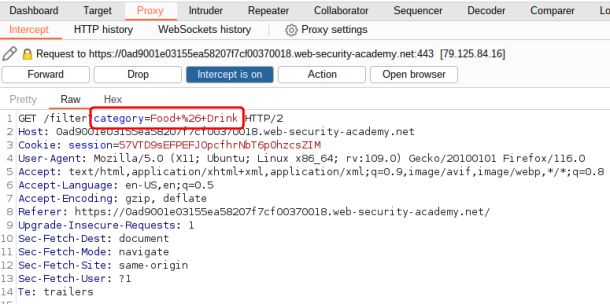
\includegraphics[width=1\linewidth]{Images//sql injection/in_intercept.png}    
    \end{figure}
    \item let append {\color{orange}\textbf{'+OR+1=1-- }} to the request like below
    \begin{figure}[H]
        \centering
        \includegraphics[width=1\linewidth]{sql_injection_in_intercept.png}
        
        
    \end{figure}
    \begin{figure}[H]
    \centering
    \includegraphics[width=0.7\linewidth]{Images//sql injection/result.png}
    
\end{figure}
\item Now we can see that, there are now even many hidden contents, which the site didn’t show us in first place.    
\end{itemize}

%----------------------------------------------------------------------------------------
%	Penetration testing workflow - Testing for vulnerabilities - Testing XSS(Cross Site Scripting) Vulnerabilities
%----------------------------------------------------------------------------------------
\addcontentsline{toc}{subsubsection}{Testing XSS Vulnerabilities}
\subsubsection*{Testing XSS(Cross Site Scripting) Vulnerabilities}

%----------------------------------------------------------------------------------------
%	Penetration testing workflow - Testing for vulnerabilities - Identifying reflected input
%----------------------------------------------------------------------------------------
\subsubsection*{Stage-1: Identifying reflected input}
Reflected input is when data is copied from a request and echoed into the 
application's immediate response. \newline
Let's test this lab : \href{https://portswigger.net/web-security/cross-site-scripting/reflected/lab-html-context-nothing-encoded}{\color{orange}reflected \textunderscore input \textunderscore lab}
\begin{figure}[H]
    \centering
    \includegraphics[width=0.75\linewidth]{Images/searchBox.png}
    
    
\end{figure}
\begin{itemize}
    \item Input anything. And go to {\color{orange}\textbf{proxy}} > {\color{orange}\textbf{http history}}. And send that request to active scan.
    \begin{figure}[H]
        \centering
        \includegraphics[width=1\linewidth]{Images//Reflected XSS/send_to_scan.png}        
    \end{figure}

    \item Look any issue arises related XSS
    \begin{figure}[H]
        \centering
        \includegraphics[width=1\linewidth]{Images//Reflected XSS/issues.png}
        
        
    \end{figure}
    \item Let's investigate the request. Send the request to the repeater.
\begin{figure}[H]
    \centering
    \includegraphics[width=1\linewidth]{Images//Reflected XSS/send_to_repeater.png}
    
    
\end{figure}
    \item Change the input field to anything.
    \begin{figure}[H]
        \centering
        \includegraphics[width=1\linewidth]{Images//Reflected XSS/something.png}       
    \end{figure}
\begin{figure}[H]
    \centering
    \includegraphics[width=1\linewidth]{Images//Reflected XSS/response-1.png}
\end{figure}

    \item So, we now know how our input is reflected. Let’s start attacking. 
    \item For this, we have to turn on the intercept. And make request from browser.
    \begin{figure}[H]
        \centering
        \includegraphics[width=0.75\linewidth]{Images//Reflected XSS/request.png}
        
        
    \end{figure}
    \begin{figure}[H]
        \centering
        \includegraphics[width=0.75\linewidth]{Images//Reflected XSS/intercaption.png}
        
    \end{figure}

    \item append {\color{orange}\textbf{<script>alert('hacked')</script>}} 
    \begin{figure}[H]
        \centering
        \includegraphics[width=1\linewidth]{Images//Reflected XSS/intercept.png}
        
    \end{figure}

    \item check the response now.

    
\end{itemize}


\end{fullwidth}









\end{document}
